\documentclass[11pt]{article}
\addtolength{\oddsidemargin}{-1.cm}
\addtolength{\textwidth}{2cm}
\addtolength{\topmargin}{-2cm}
\addtolength{\textheight}{3.5cm}
\newcommand\tab[1][1cm]{\hspace*{#1}}
\usepackage[pdftex]{graphicx}
\usepackage{pdflscape}
\usepackage[T1]{fontenc}
\usepackage{hyperref}
\usepackage{float}
\usepackage{cite}

\hypersetup{
	colorlinks=true,
	linkcolor=black,
	filecolor=magenta,
	urlcolor=cyan,
}

% define the title
\author{Binary Ninjaz}
\title{Harvest}
\begin{document}
\begin{titlepage}

	\begin{center}
		% Upper part of the page
		\textsc{\LARGE Binary Ninjaz}\\[0.3cm]
		% Title
		\rule{\linewidth}{0.5mm} \\[0.5cm]
		{ \huge \bfseries Harvest \\
		  \vspace{0.3cm}\large \bfseries User Manual}\\[0.5cm]
		\rule{\linewidth}{0.5mm} \\[1cm]


		\begin{minipage}{0.4\textwidth}
			\begin{flushleft} \large
				\emph{} \\
				Letanyan {Arumugam}
			\end{flushleft}
		\end{minipage}
		\begin{minipage}{0.4\textwidth}
			\begin{flushright} \large
				\emph{} \\
				14228123
			\end{flushright}
		\end{minipage}

		\begin{minipage}{0.4\textwidth}
			\begin{flushleft} \large
            	\emph{} \\
				Sizo {Duma}
			\end{flushleft}
		\end{minipage}
		\begin{minipage}{0.4\textwidth}
			\begin{flushright} \large
				\emph{} \\
				15245579
			\end{flushright}
		\end{minipage}

		\begin{minipage}{0.4\textwidth}
			\begin{flushleft} \large
				\emph{} \\
				Teboho {Mokoena}
			\end{flushleft}
		\end{minipage}
		\begin{minipage}{0.4\textwidth}
			\begin{flushright} \large
				\emph{} \\
				14415888
			\end{flushright}
		\end{minipage}

		\begin{minipage}{0.4\textwidth}
			\begin{flushleft} \large
				\emph{} \\
				John {Ojo}
			\end{flushleft}
		\end{minipage}
		\begin{minipage}{0.4\textwidth}
			\begin{flushright} \large
				\emph{} \\
				15096794
			\end{flushright}
		\end{minipage}

        \begin{minipage}{0.4\textwidth}
			\begin{flushleft} \large
				\emph{} \\
				Kevin {Reid}
			\end{flushleft}
		\end{minipage}
		\begin{minipage}{0.4\textwidth}
			\begin{flushright} \large
				\emph{} \\
				15008739
			\end{flushright}
		\end{minipage}
        
        \begin{minipage}{0.4\textwidth}
			\begin{flushleft} \large
				\emph{} \\
				Shaun {Yates}
			\end{flushleft}
		\end{minipage}
		\begin{minipage}{0.4\textwidth}
			\begin{flushright} \large
				\emph{} \\
				16007493
			\end{flushright}
		\end{minipage}

		\vspace{1cm}
		\rule{\linewidth}{0.5mm} \\[1cm]
		\textsc{\Large Stakeholders}\\[1cm]

		\begin{minipage}{0.4\textwidth}
			\begin{flushleft} \large
				\emph{} \\
				SAMAC:
			\end{flushleft}
		\end{minipage}
		\begin{minipage}{0.4\textwidth}
			\begin{flushright} \large
				\emph{} \\
				Barry Christie
			\end{flushright}
		\end{minipage}


	\end{center}
\end{titlepage}

\newpage
\pagenumbering{Roman}
\tableofcontents
\newpage
\listoffigures

\newpage
\pagenumbering{arabic}

\section{General Information}
\subsection{System Overview}
Harvest, is an application to assist growers with yield data and optimise worker performance. In other words, it is a system that can efficiently measure the amount of work done by a worker, track the foremen on a farm, record information and data, and display the necessary information. This system is aimed at farming communities to help then record data and get work done more efficiently.

\subsection{System Requirements}
\subsubsection{Android}
The Android application currently requires:
\begin{itemize}
	\item Either Android 4.0 OS or above
\item 200 MB RAM
\item 50 MB Disk Space	
	\item Location Services
\end{itemize}
\subsubsection{iOS}
The iOS application currently requires:
\begin{itemize}
	\item iOS 10.0 or above
\item 200 MB RAM
\item 50 MB Disk Space	
	\item Location Services
\end{itemize}
\subsubsection{Website}
The website requires any modern up-to-date web browser such as Firefox, Opera, Chrome, Safari, Vivaldi, Edge, or any other.

\subsection{Communications}
All of the subsystems---Android, iOS, and website---run independently, but use Firebase\footnote{\url{https://firebase.google.com}} to store and retrieve data from a common source. This can be seen in \ref{Communications}

\begin{figure}
 \centering
 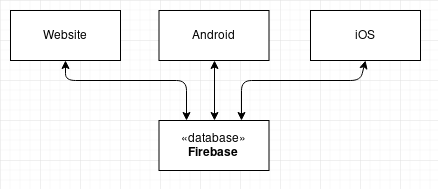
\includegraphics[width=12cm, keepaspectratio]{Images/webDiagramCommunications.png}
 \caption{Communications}
 \label{Communications}
\end{figure}

\subsection{Installation}
\subsubsection{Android}
The application will be available for download on the Google Play Store.
\subsubsection{iOS}
The application will be available for download on the Apple App Store.
\subsubsection{Website}
No Installation is required to use the website, however it can be accessed at <Web Link>.
\subsubsection{Location Services}
With regards to configuring the iOS and Android applications: location services are required. The user will be prompted for the location permissions in mention to allow full functionality of the application. Profile setting can be configured via selecting the user's username.

\newpage
\section{Getting Started}
\textit{From this point on, the functioning of the Android and iOS applications are similar, so they are grouped into a single} Mobile \textit{section, and unless otherwise stated, the description applies to both applications.}

\subsection{Mobile}

\subsubsection{Creating an Account}
The application will open by default on the log in screen. From here the user can choose to sign in as a farmer or as a foreman, or to create a new farmer account. A foreman does not need to create an account, they simply sign in with their phone number, however the farmer must ensure that the foreman appears on their system and that the foreman's number is correct.\\
To create a farmer account the following information is required:
\begin{itemize}
\item Email
\item Password
\end{itemize}
Additionally the following information can be optionally provided:
\begin{itemize}
\item First name
\item Surname
\item Organization
\end{itemize}
Organization is most important since it will be used by foremen to identify your organization when they log in. \textbf{If it is not provided, you will be identified by your email, which will then be visible to your foremen.}

\begin{figure}[h]
 \centering
 \includegraphics[width=6cm, keepaspectratio]{Images/mobileLoginChoose.png}
 \caption{Sign In/Up Method Choose}
 \label{SignUpMobile}
\end{figure}

\subsubsection{Logging In as a Farmer}
When on the log in screen enter your email and its password you used to create the account, alternatively click log in with Google to use Google credentials, which will be linked to Harvest if they have not already. If you have already logged in the app will keep you logged in until you log out.
\begin{figure}[h]
 \centering
 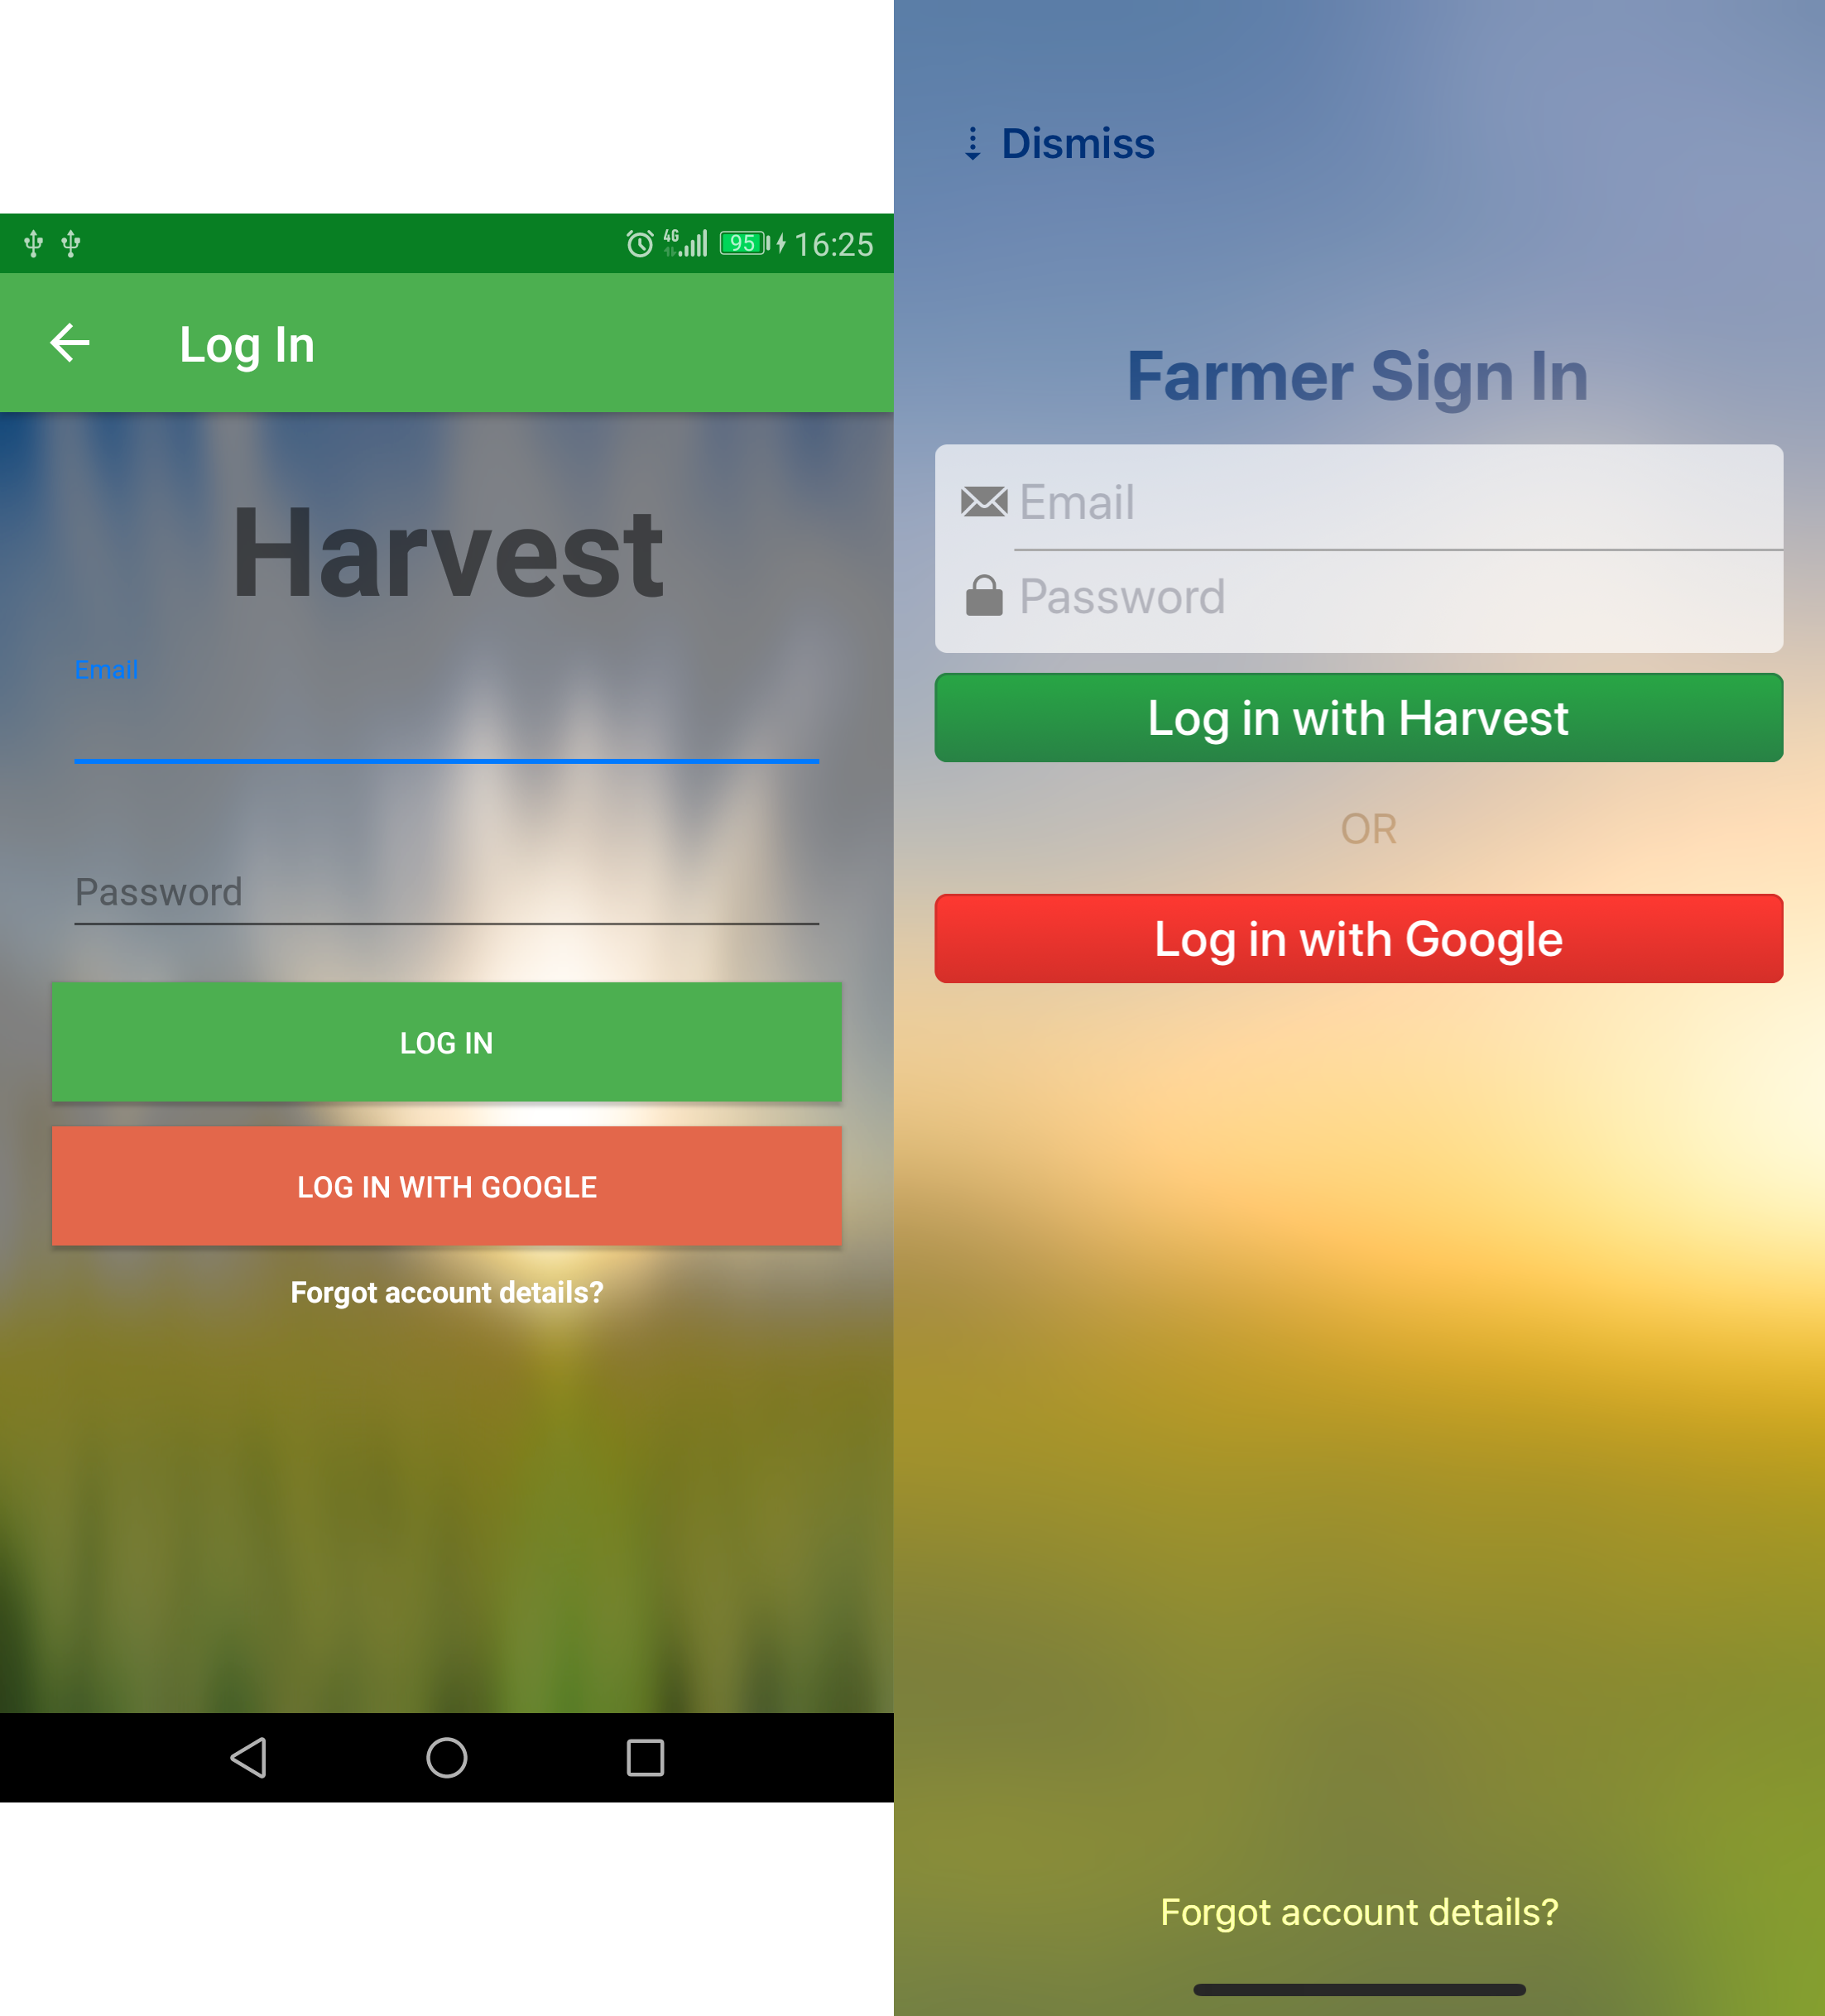
\includegraphics[width=6cm, keepaspectratio]{Images/mobileLoginFarmer.png}
 \caption{Log In Form for Farmer}
 \label{LogInMobile}
\end{figure}

\subsubsection{Logging In as a Foreman}

Simply enter your mobile phone number and press the button. A verification code may be sent to you via SMS, which will then need to be entered. Once that is done a confirmation screen will be displayed, it will show the phone number saved in the system so that the farmer can confirm that it is saved correctly. Then, depending on the situation, the following will be displayed:
\begin{itemize}
 \item If the foreman is not assigned to any organization, then they will be prompted to go back and will not be able to continue.
 \item If the foreman is assigned to a single organization, the name will be displayed, and they will then be able to continue to the clicker as seen in \ref{Clicker}.
 \item On the off chance that the foreman is assigned to multiple organizations, they will be able to select which organization they wish to work for for the session. In order to change this, they must log out and in again.
\end{itemize}

\subsubsection{Logging Out}
The Log out button can be found at the bottom of the Harvest "Settings" Tab.

\subsection{Website}



\textit{For ease of visualization, a diagram representing a map of the website is given in \ref{WebsiteMap}: each web page is given, indicating to where, and how a traversal is possible from that page.}

\begin{figure}[h]
 \centering
 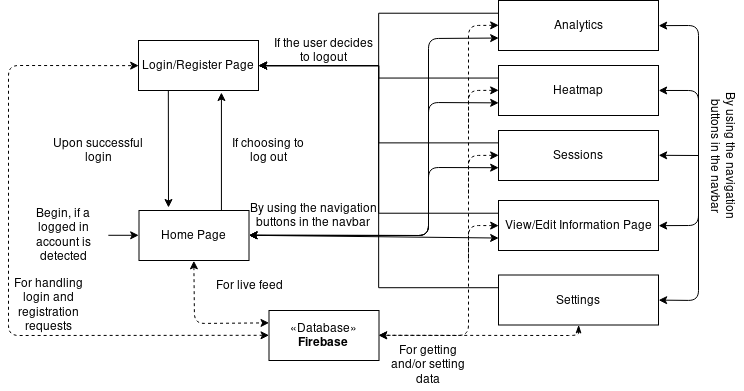
\includegraphics[width=12cm, keepaspectratio]{Images/webDiagramMap.png}
 \caption{Website Map}
 \label{WebsiteMap}
\end{figure}

\subsubsection{Registering}
\paragraph{Finding the Register Page}The login and registration page can be found at <Web Link>, and once there the user will be presented with the page as seen in \ref{LoginPage}. To now create an account the user must click on the blue \texttt{Don't have an account? Sign Up} button. They will now be presented with the above page.

\begin{figure}
 \centering
 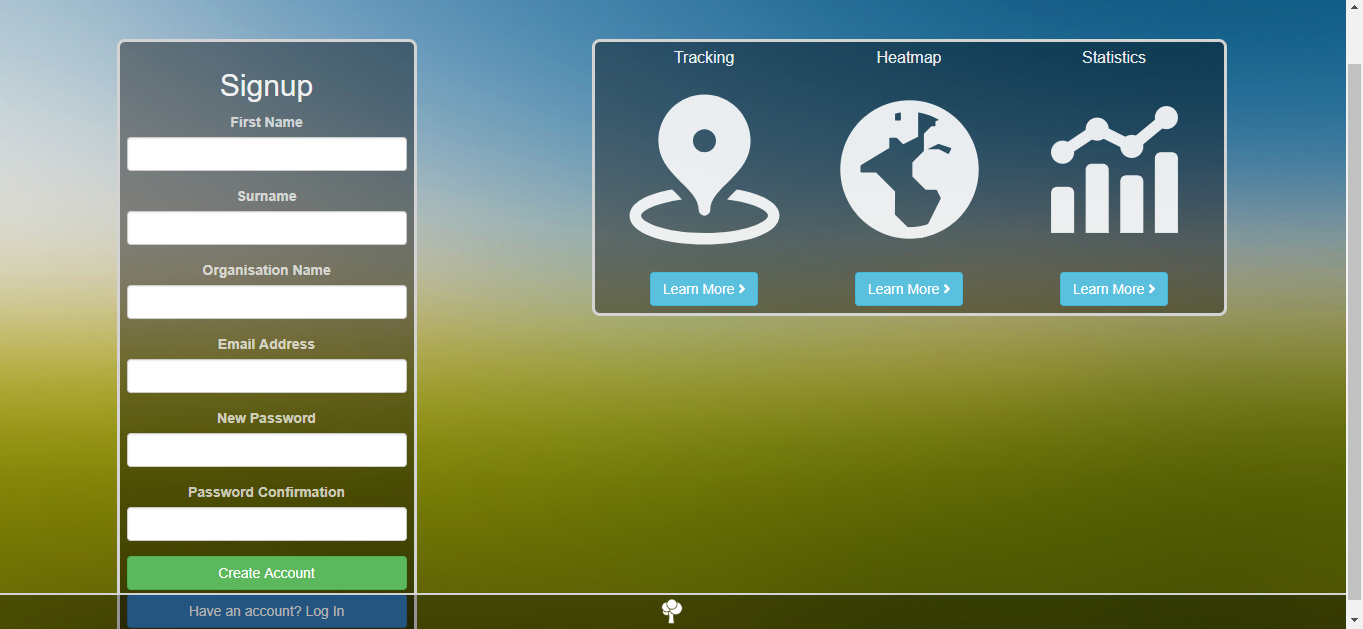
\includegraphics[width=12cm, keepaspectratio]{Images/webRegister-Page.png}
 \caption{Register Page}
 \label{RegisterPage}
\end{figure}

\paragraph{Creating an Account}Once at the register page the new user must enter their first name, surname, email address, desired password, and confirm the desired password by entering it again. When all of the information has been entered, and the user is content that the information is correct, they shall click on the green \texttt{Create Account} button. They will now be taken to the login page as seen in \ref{LoginPage}. The user shall receive an email as seen in \ref{AccountCreationConfirmationEmail} at the specified address, asking to confirm their account. The user simply needs to click on the \texttt{Confirm Account} button in order to complete the account creation.

\subsubsection{Logging In}
\paragraph{Finding the Login Page}The login and register page can be found at <Web Link>.

\begin{figure}
 \centering
 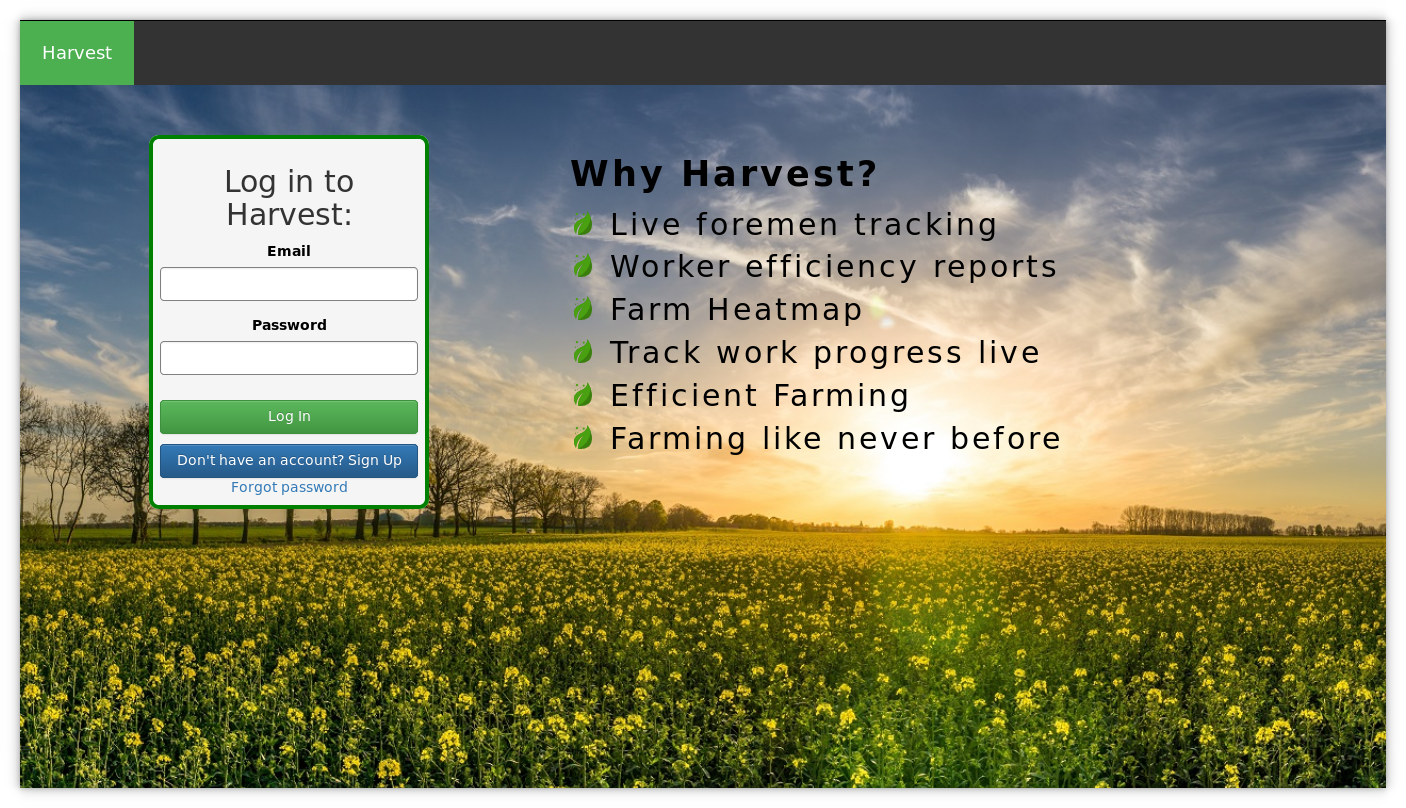
\includegraphics[width=12cm, keepaspectratio]{Images/webLogin.png}
 \caption{Login Page}
 \label{LoginPage}
\end{figure}

\paragraph{Logging In}The user simply enters the correct email address and password associated with their account, and clicks on the green \texttt{Log In} button. The user will the now be taken to \ref{webHome}.

\subsubsection{Logging Out}
\label{webLoggingOut}
The \texttt{Sign Out} button can be clicked, at the top right of the navigation bar, to sign out at any time.

\newpage
\section{Using the System}

\subsection{Mobile}
\subsubsection{Navigating}
If a foreman is logged in, then they can only access the clicker.\\
A farmer will have a navigation bar displayed at the bottom that they can use to get to different functionalities of the application.\\
\\
\textit{A discrepancy between iOS and Android exists in the form of settings. To access the settings in Android, the three dots must be pressed on, in the top right, and settings chosen.}\\
\\
The following is accessable through the navigation bar:
\begin{itemize}
\item \ref{Mobile Yield Tracker}: Yield Tracker
\item \ref{Mobile Information}: Information
\item \ref{Mobile Sessions}: Sessions 
\item \ref{Mobile Statistics}: Statistics
\item \ref{Mobile Settings}: Settings (OS dependent)
\end{itemize}
\subsubsection{Using the Yield Tracker}
\label{Mobile Yield Tracker}

\begin{figure}
 \centering
 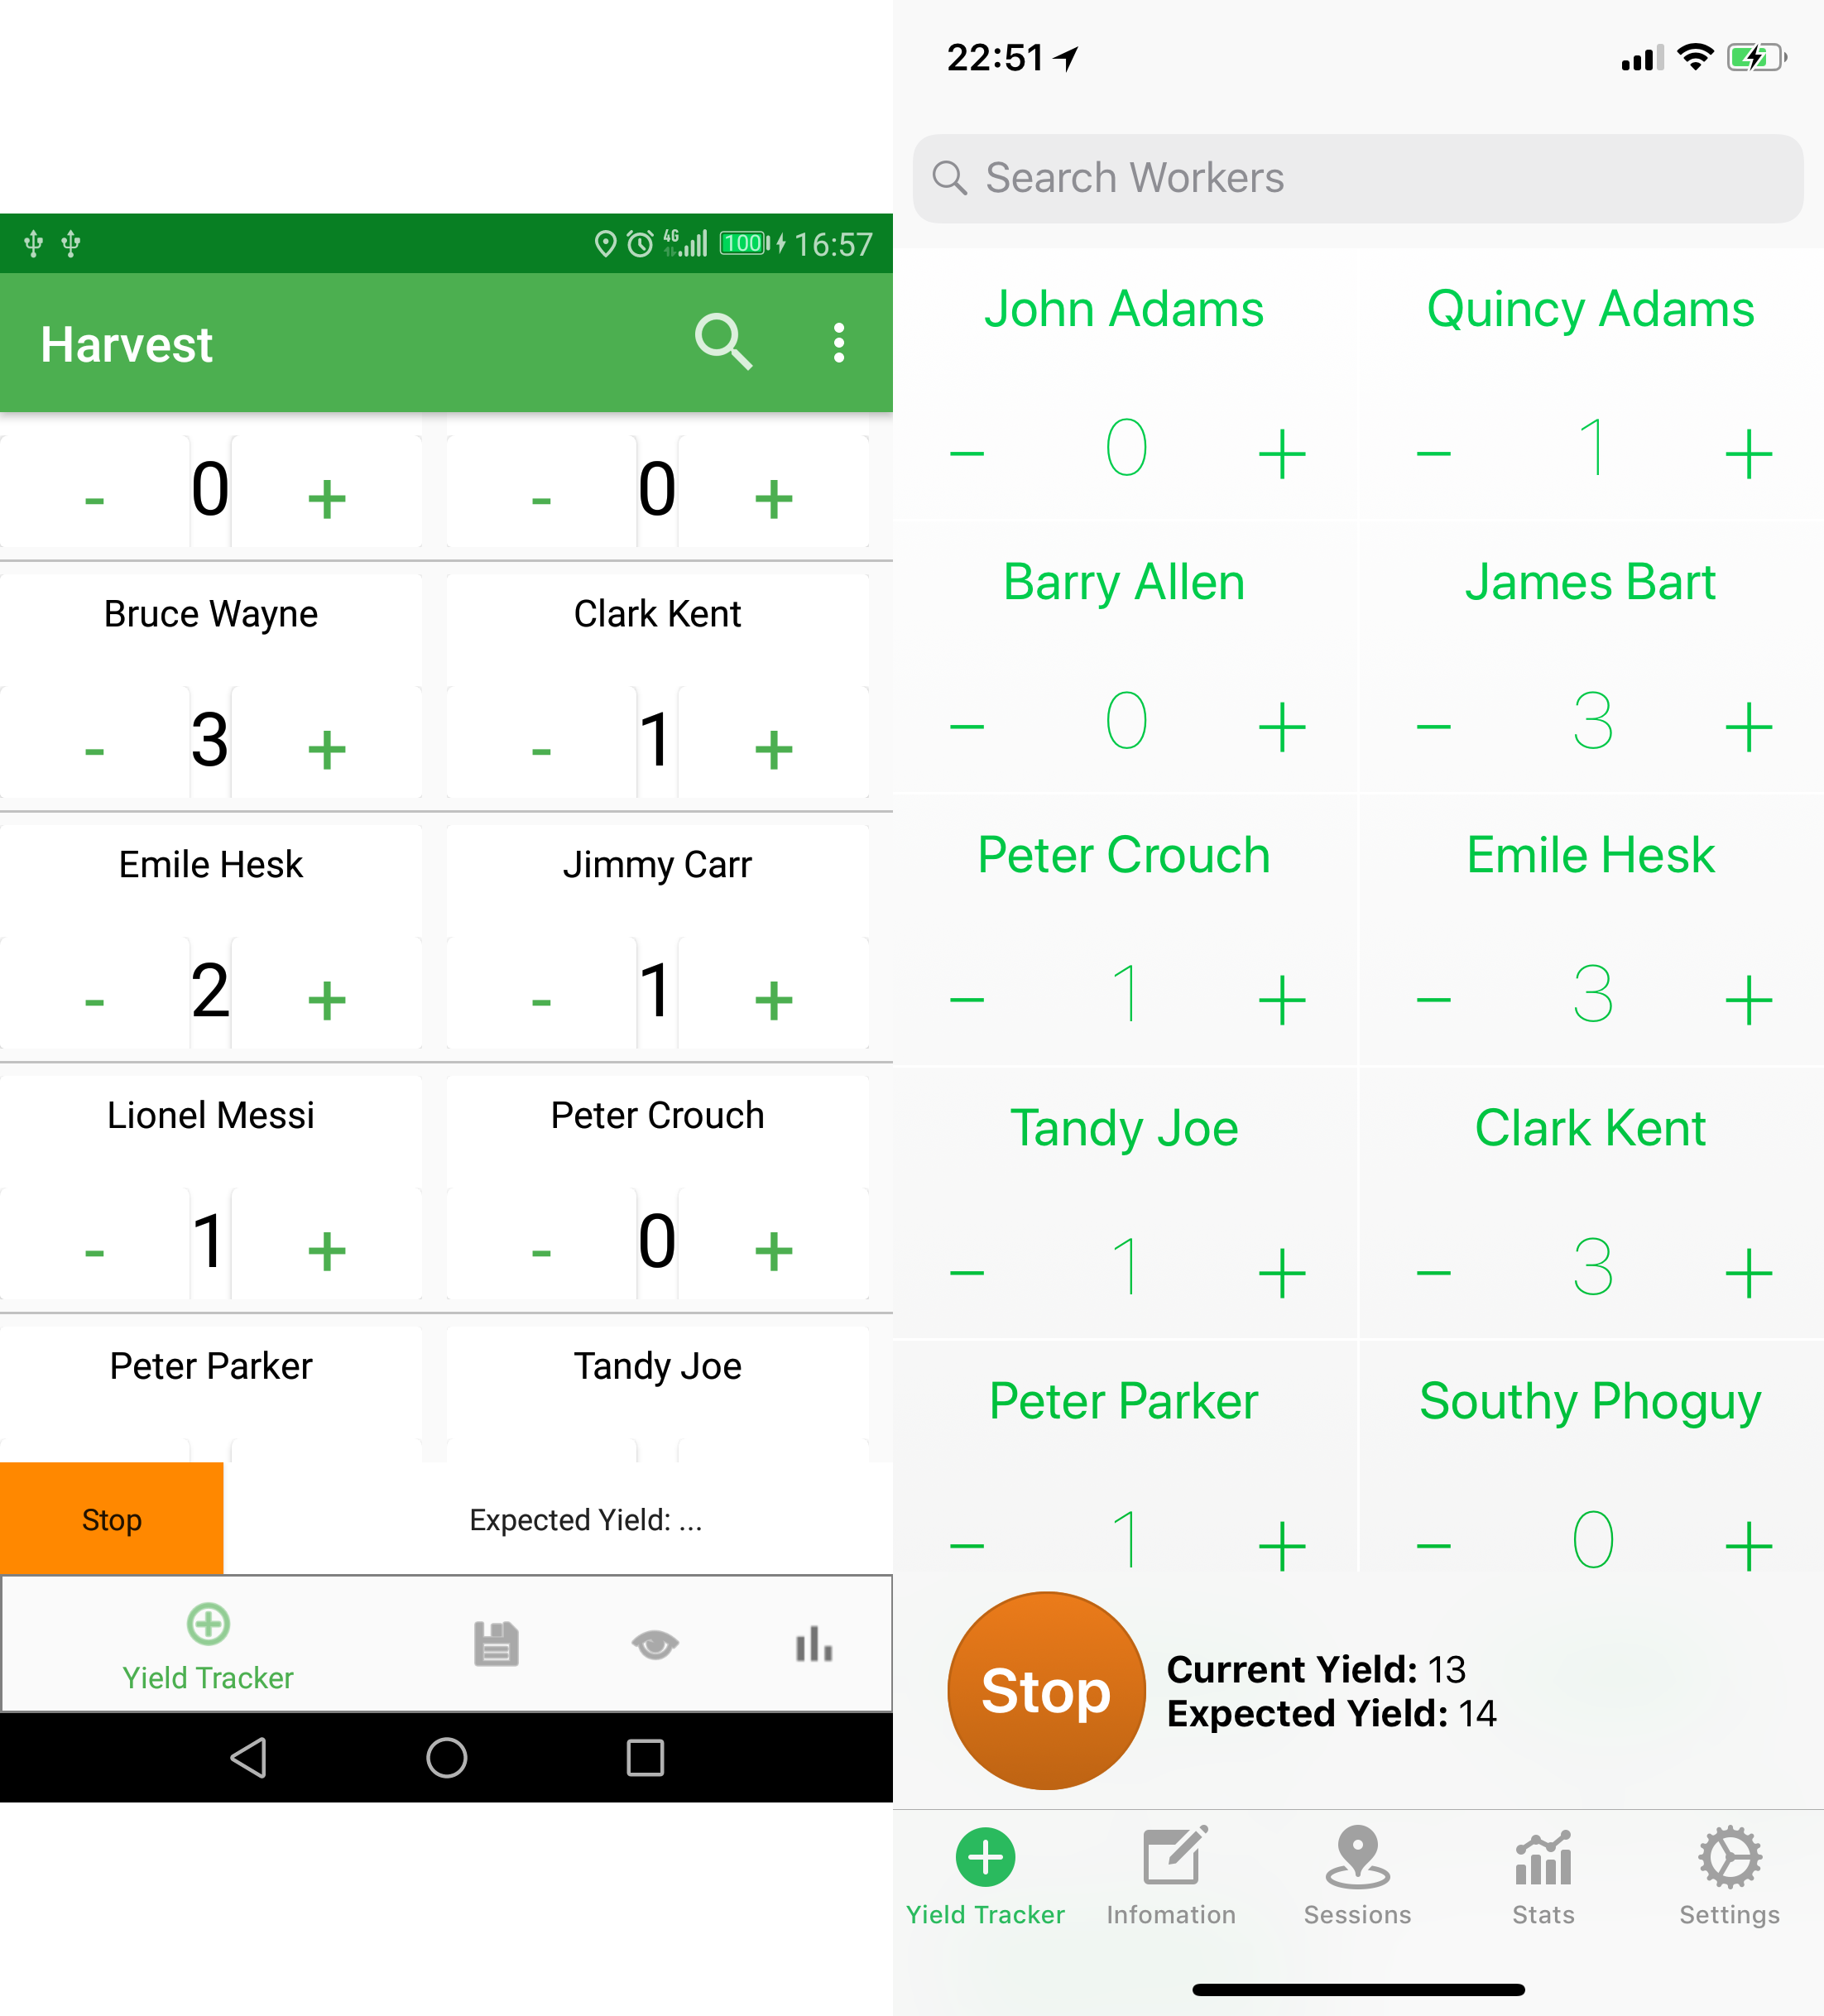
\includegraphics[width=12cm, keepaspectratio]{Images/mobileClicker.png}
 \caption{Yield Tracker}
 \label{Yield Tracker}
\end{figure}

The Yield Tracker is shown in \ref{Yield Tracker}. Should the required location permission be disallowed, and the GPS disabled, then this system will not work. The user will be prompted to enable this services.\\
Note that the bar at the bottom is only displayed when a farmer is logged in. A foreman will have no access to the other functionalities of the application.\\
\\
To use the Yield Tracker the following process is followed:
\begin{enumerate}
\item Press "Start"
\item Click the plus buttons bellow the workers name to increment or decrement the amount of bags they dropped off.
\item Press "Stop"
\item A summary of the session will be displayed.
\item The session can then be saved or discarded.
\end{enumerate}

\subsubsection{Information}
\label{Mobile Information}
This works exactly the same way as in the website, please see \ref{Web Information}.\\
Please see, however, \ref{Android Information Buttons}, for a description of unlabled buttons with regards to Information on Android. Whereby:
\subparagraph{Add} creates a new item.
\subparagraph{Save} saves the item that is being modified.
\subparagraph{Edit} allows for editing of the currently displayed item.
\subparagraph{Delete} deletes the item that is being edited. A conformation will be displayed.

\begin{figure}
 \centering
 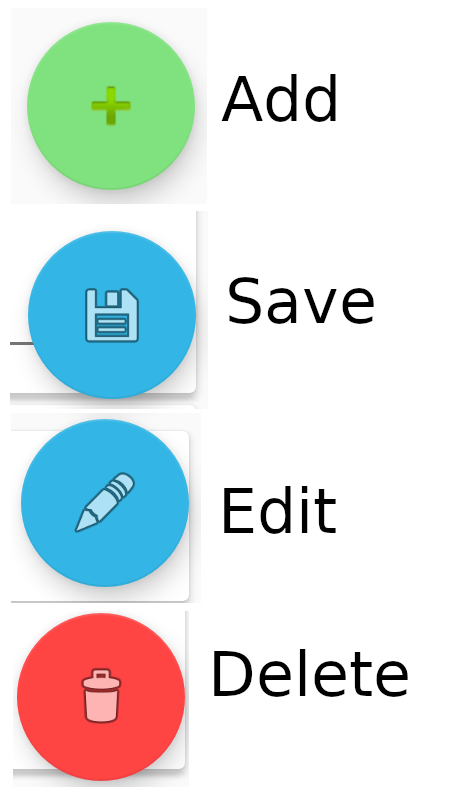
\includegraphics[width=12cm, keepaspectratio]{Images/AndroidInformationButtons.png}
 \caption{Android Information Buttons}
 \label{Android Information Buttons}
\end{figure}

\subsubsection{Sessions}
\label{Mobile Sessions}

\begin{figure}
 \centering
 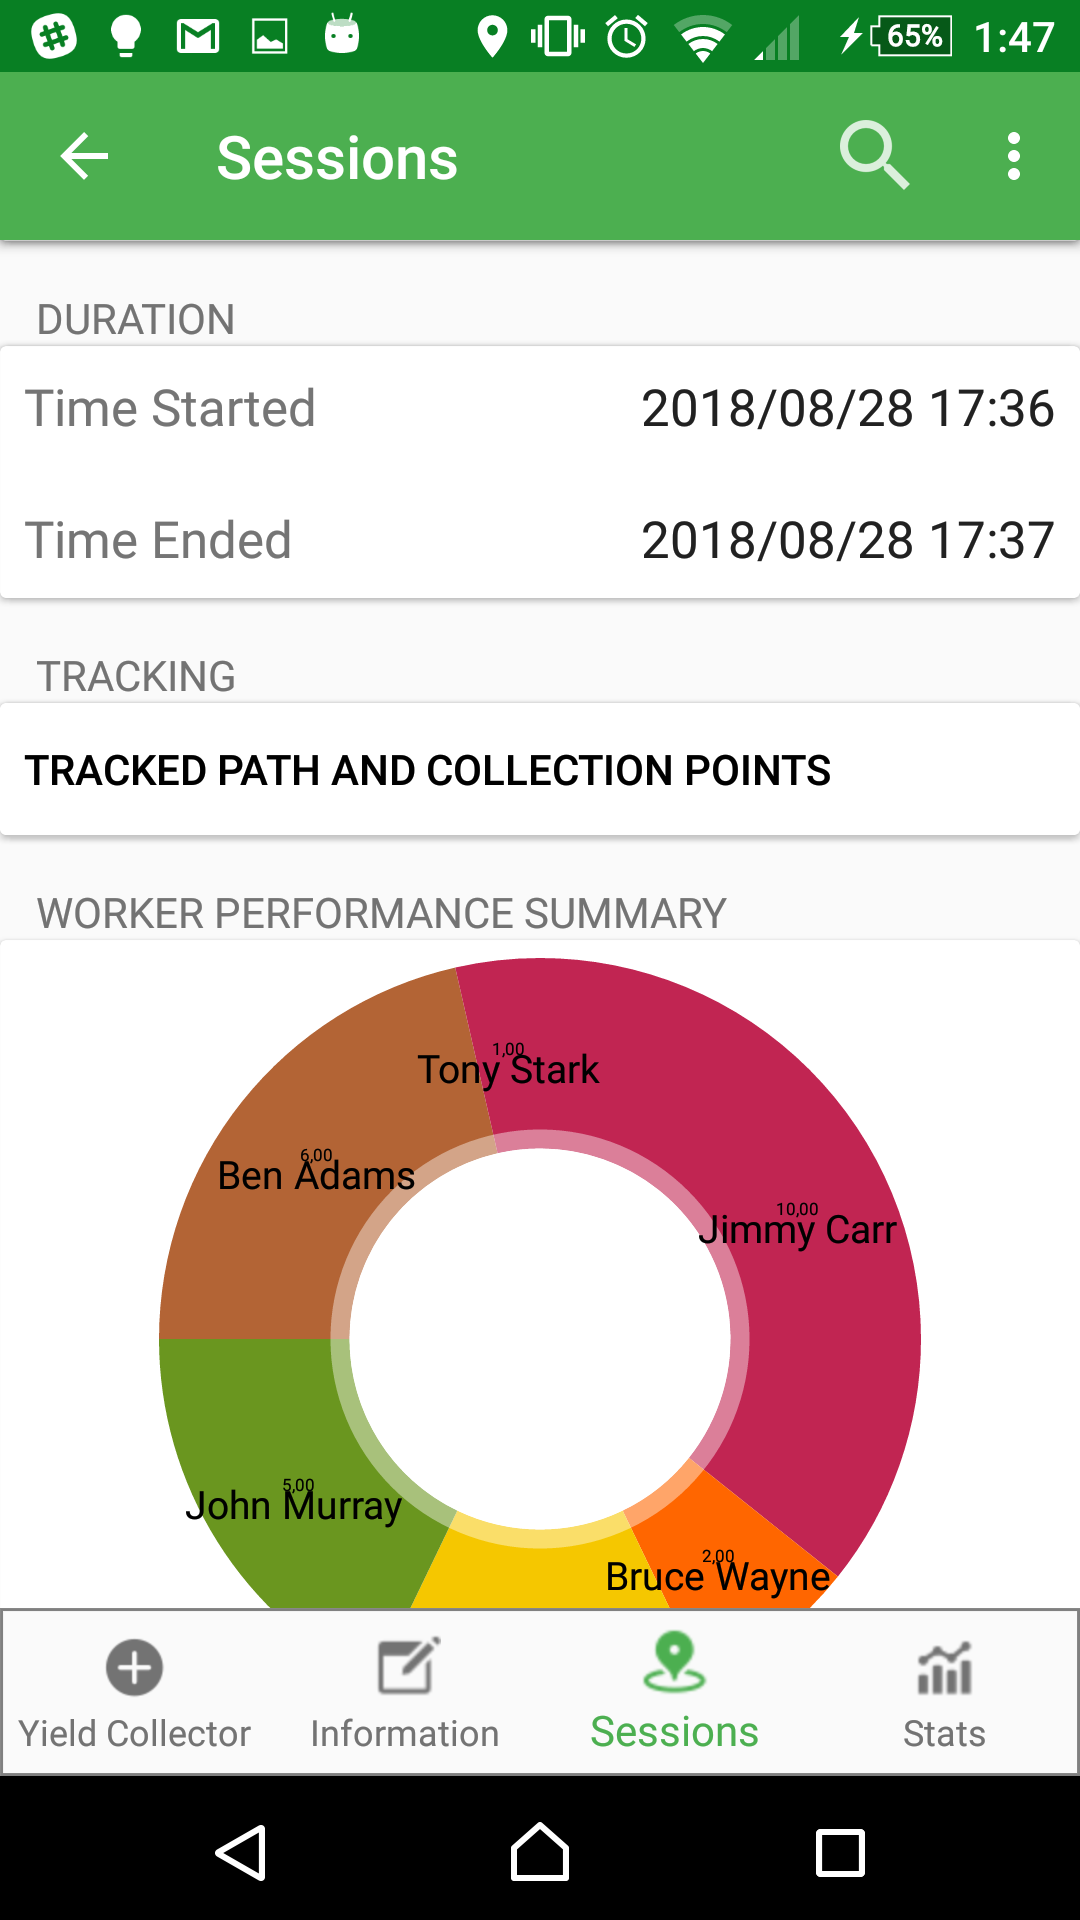
\includegraphics[width=12cm, keepaspectratio]{Images/mobileSession.png}
 \caption{Session}
 \label{Mobile Session}
\end{figure}

Here a list of all sessions carried out is displayed. A session can be selected to get retrieve further information about it. See \ref{Mobile Session}. The button \texttt{TRACKED PATH AND COLLECTION POINTS} can be selected to see a map, where all of the orchards can be seen, as well as the path that was taken by the foreman that was administering the session. Red pins can also be seen along the path, where each indicates where the foreman was when they indicated a bag dropped by a worker.

\subsubsection{Statistics}
\label{Mobile Statistics}

From here, varies statistics can be seen.

\subsubsection{Settings}
\label{Mobile Settings}

The following settings are available:
\begin{itemize}
 \item Account: account related settings.
 \begin{itemize}
  \item Update Email: change email address (may need to re-authorize.)
  \item Update Password: change password (may need to re-authorize.)
  \item Organization: change the name of the organization, used by foremen to identify it.
  \item First Name: change first name.
  \item Surname: change surname.
  \item Delete Account: delete the account. \textbf{This is irreversible, all information related to the account will be lost} (may need to re-authorize.)
 \end{itemize}
 \item Logout (iOS only, on android this is accessed from the menu that is used to access settings.)
\end{itemize}
\textit{Some sensitive settings, such as deleting the account, may require the user to re-authorize. In this scenario, a dialog will pop up asking them to re-enter their email and password; after which the action will be performed.}

\subsection{Website}
\subsubsection{Navigating}
\label{webNavigating}
On all web pages a consistent navbar can be seen at the top of the page. The following items are always present:
\begin{itemize}
 \item \ref{webHome}: Home Page
 \item \ref{webInformation}: Information
 \item \ref{webSessions}: Sessions
 \item \ref{webHeatmap}: Heatmap
 \item \ref{webAnalytics}: Analytics
 \item \ref{webSettings}: Settings
 \item \ref{webLoggingOut}: Sign Out
\end{itemize}
\subsubsection{Home Page}
\label{webHome}
Once the user has logged in, they will be taken to the home page, as seen in \ref{HomePage}. The home page is the starting point of the system, it serves simply by providing a real time updating feed of all bag drops, and a map overview of the farm and the locations of foremen.

\begin{figure}
 \centering
 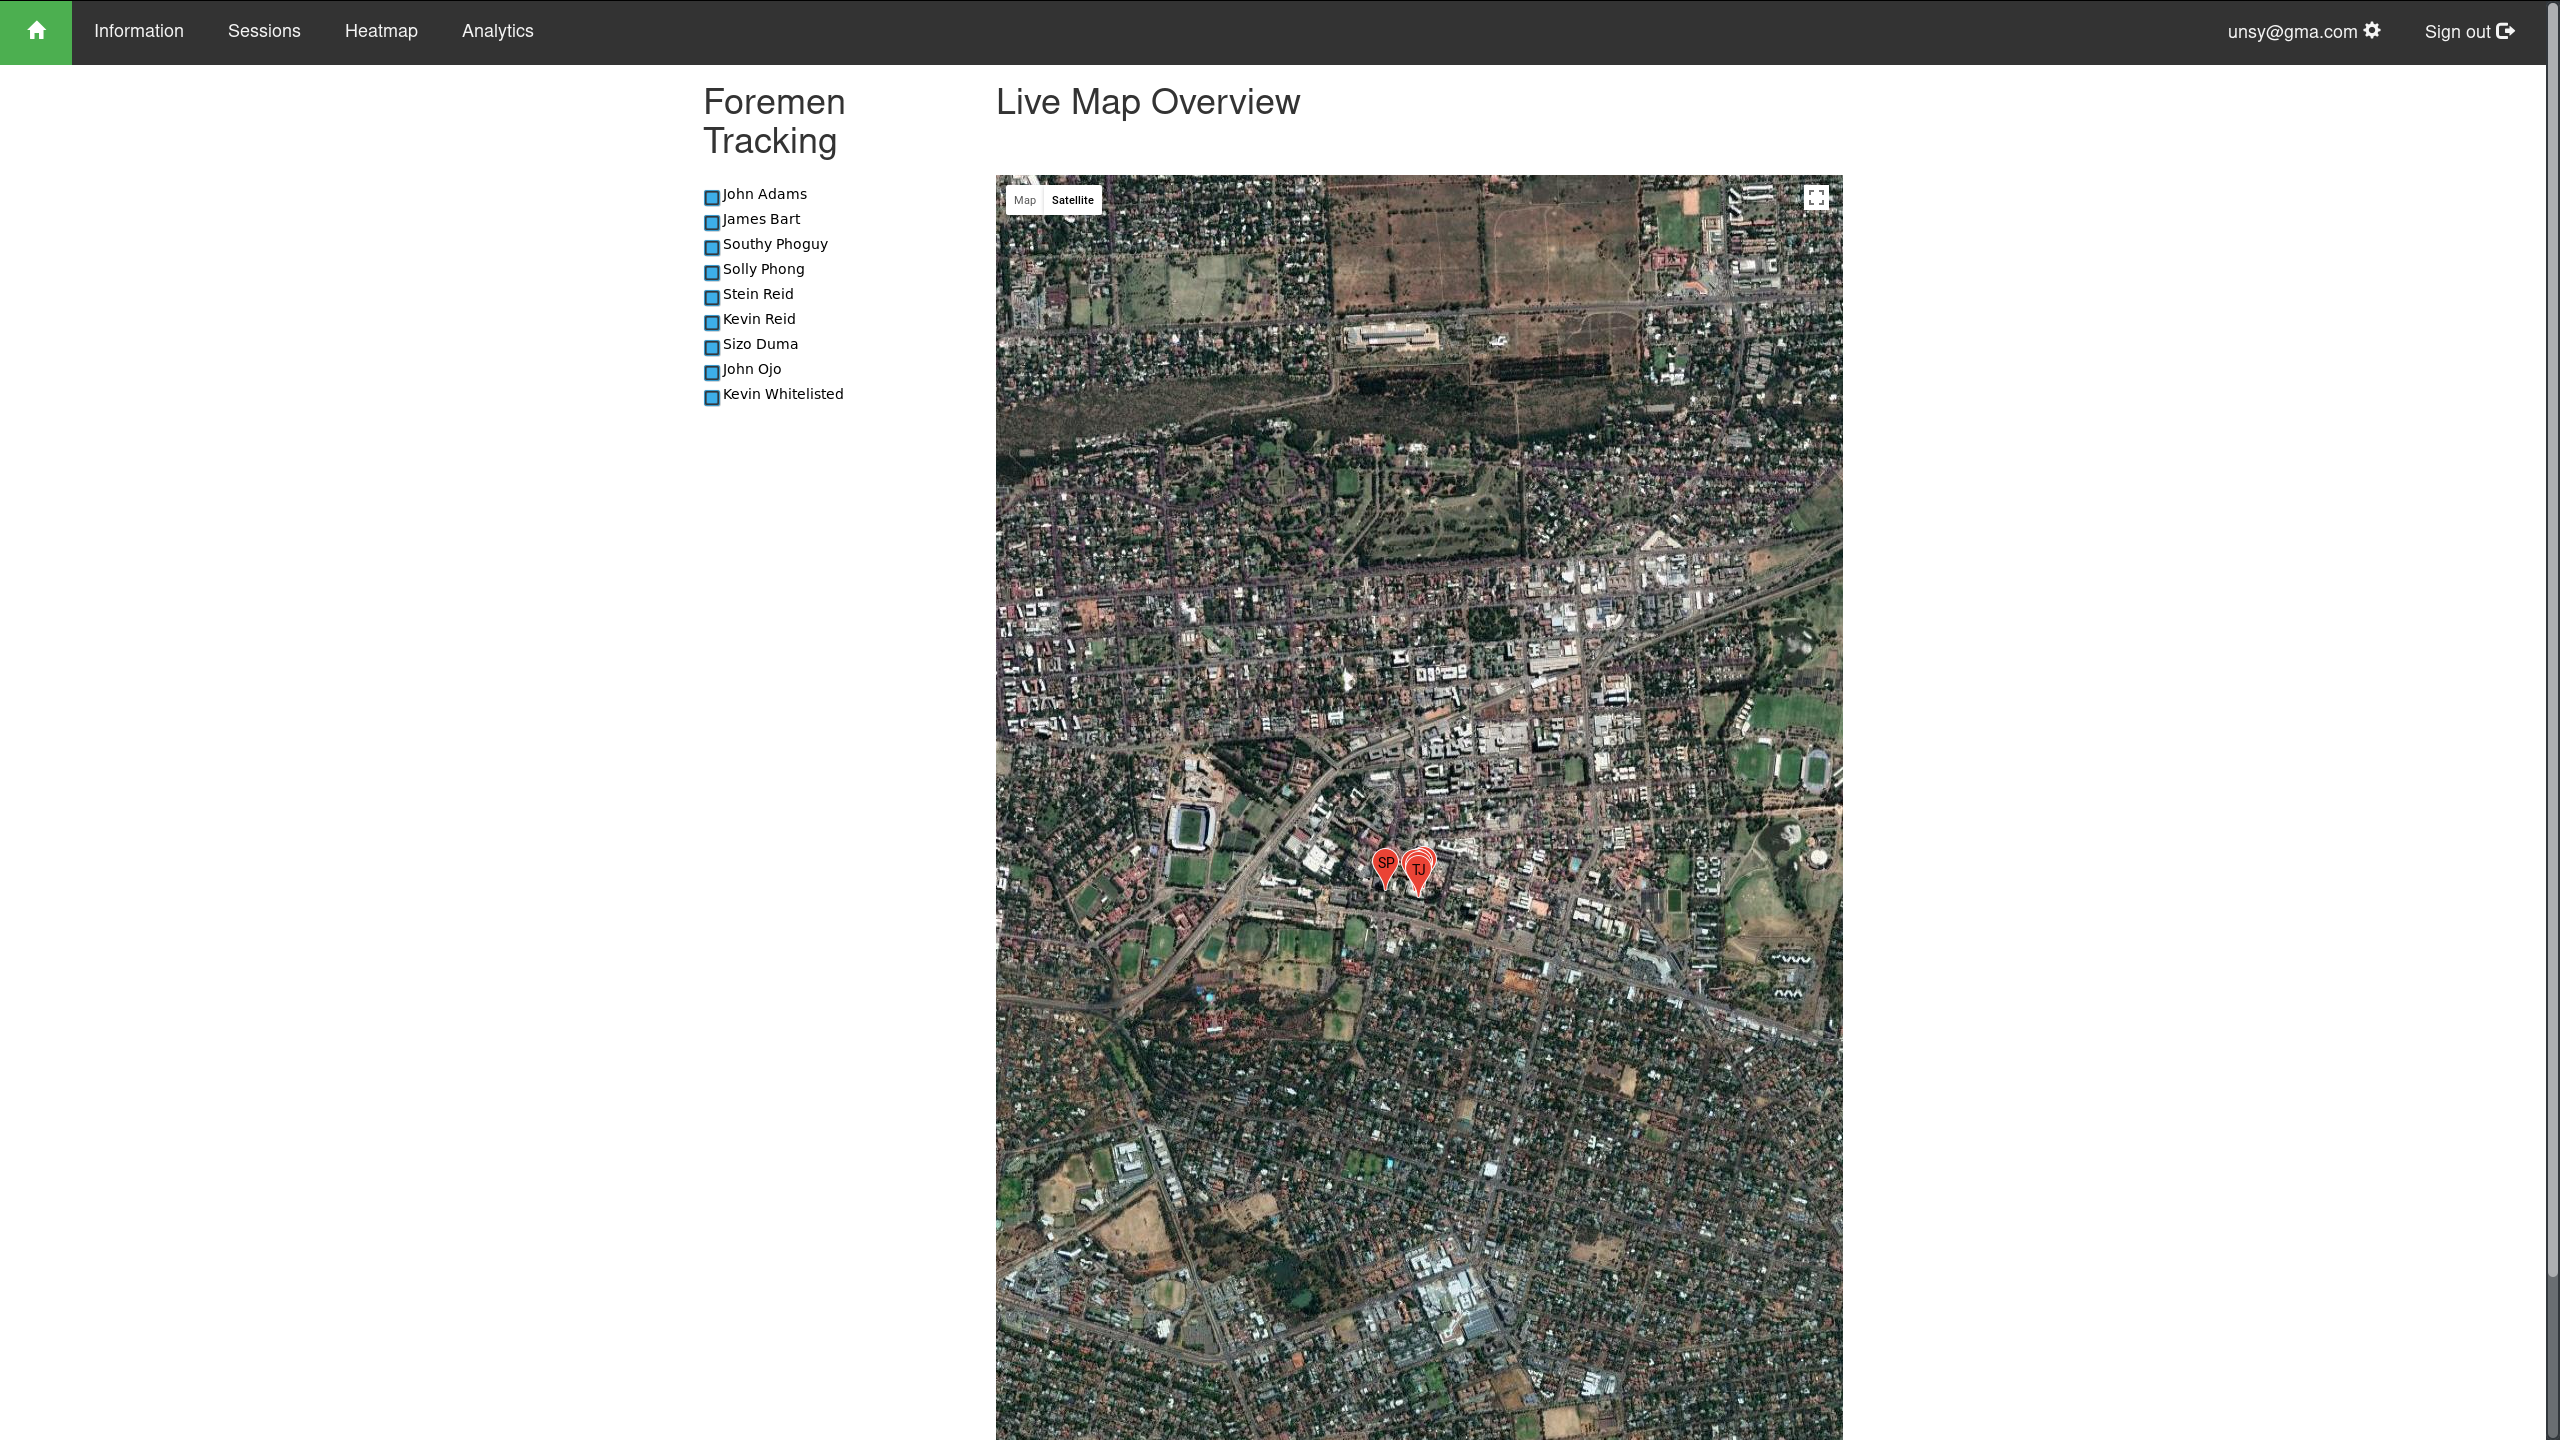
\includegraphics[width=12cm, keepaspectratio]{Images/webHome-Page.png}
 \caption{Home Page}
 \label{HomePage}
\end{figure}

\subsubsection{View/Edit Information}
\label{webInformation}
\paragraph{Introduction}The View/Edit Information page can be found at any time by clicking on the \texttt{View/Edit Information} button in the navbar. Once clicked on, the user will be taken to \ref{InformationPage}. The concept is that almost all information can be viewed from this page, and once the relevant information has been located, it can also be edited.

\begin{figure}
 \centering
 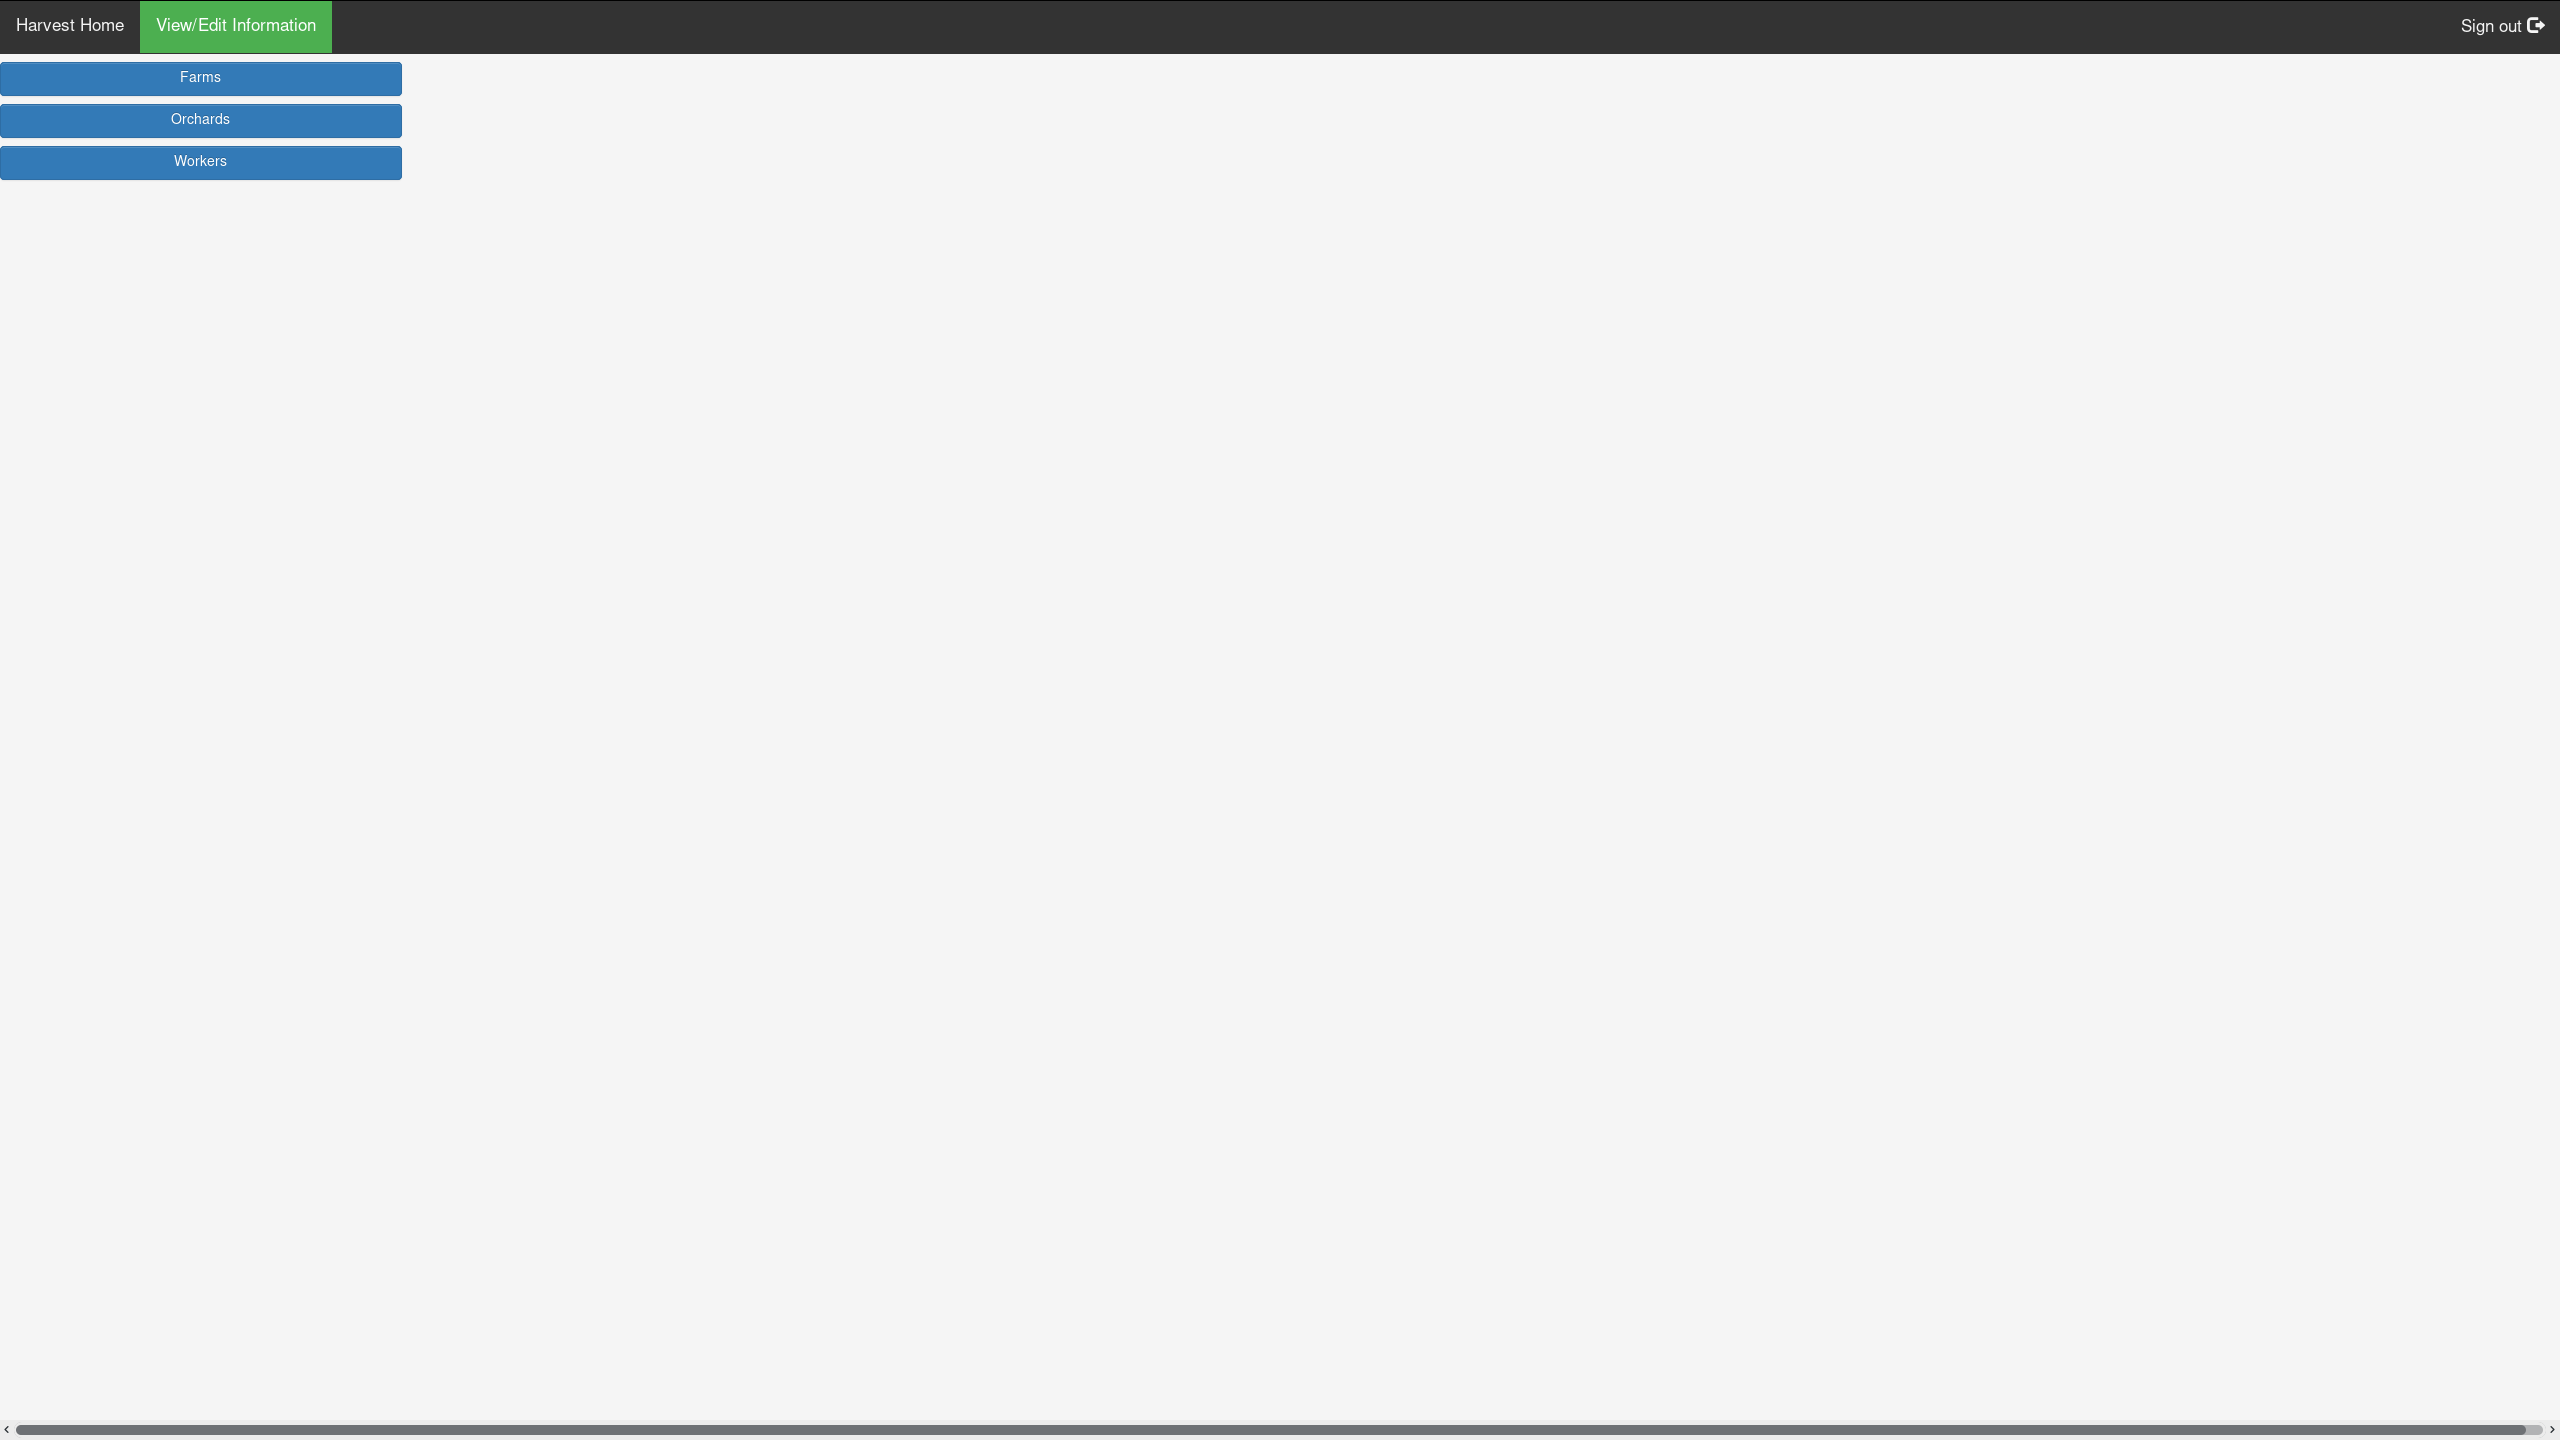
\includegraphics[width=12cm, keepaspectratio]{Images/webInformation-Page.png}
 \caption{View/Edit Information Page}
 \label{InformationPage}
\end{figure}

\paragraph{Locating the Correct Information}When in \ref{InformationPage} there are three blue buttons available; \texttt{Farms}, \texttt{Orchards}, and \texttt{Workers}. Each of which will expand a list of the relevant items. The entire process is best described through an example, so, in this example, the goal is to locate information on a worker named \textit{Joe Soap}. The process, however can be accomplished in multiple ways; the first, and most obvious is to select \texttt{Workers}, then \texttt{J. Soap} (the process can be seen by following \ref{InformationPage}, \ref{InformationPageWorkers}, and \ref{InformationPageJoe}), however, if the user is looking at the \texttt{Pear Shaped} orchard, and see's that \textit{Joe Soap} is assigned (see \ref{InformationPagePear}), then they can click on the button representing \textit{Joe Soap}---labeled \texttt{J. Soap}---to go to \textit{Joe Soap's} page, as seen in \ref{InformationPageJoePear}, note that the list of orchards is still displayed.

\begin{figure}
 \centering
 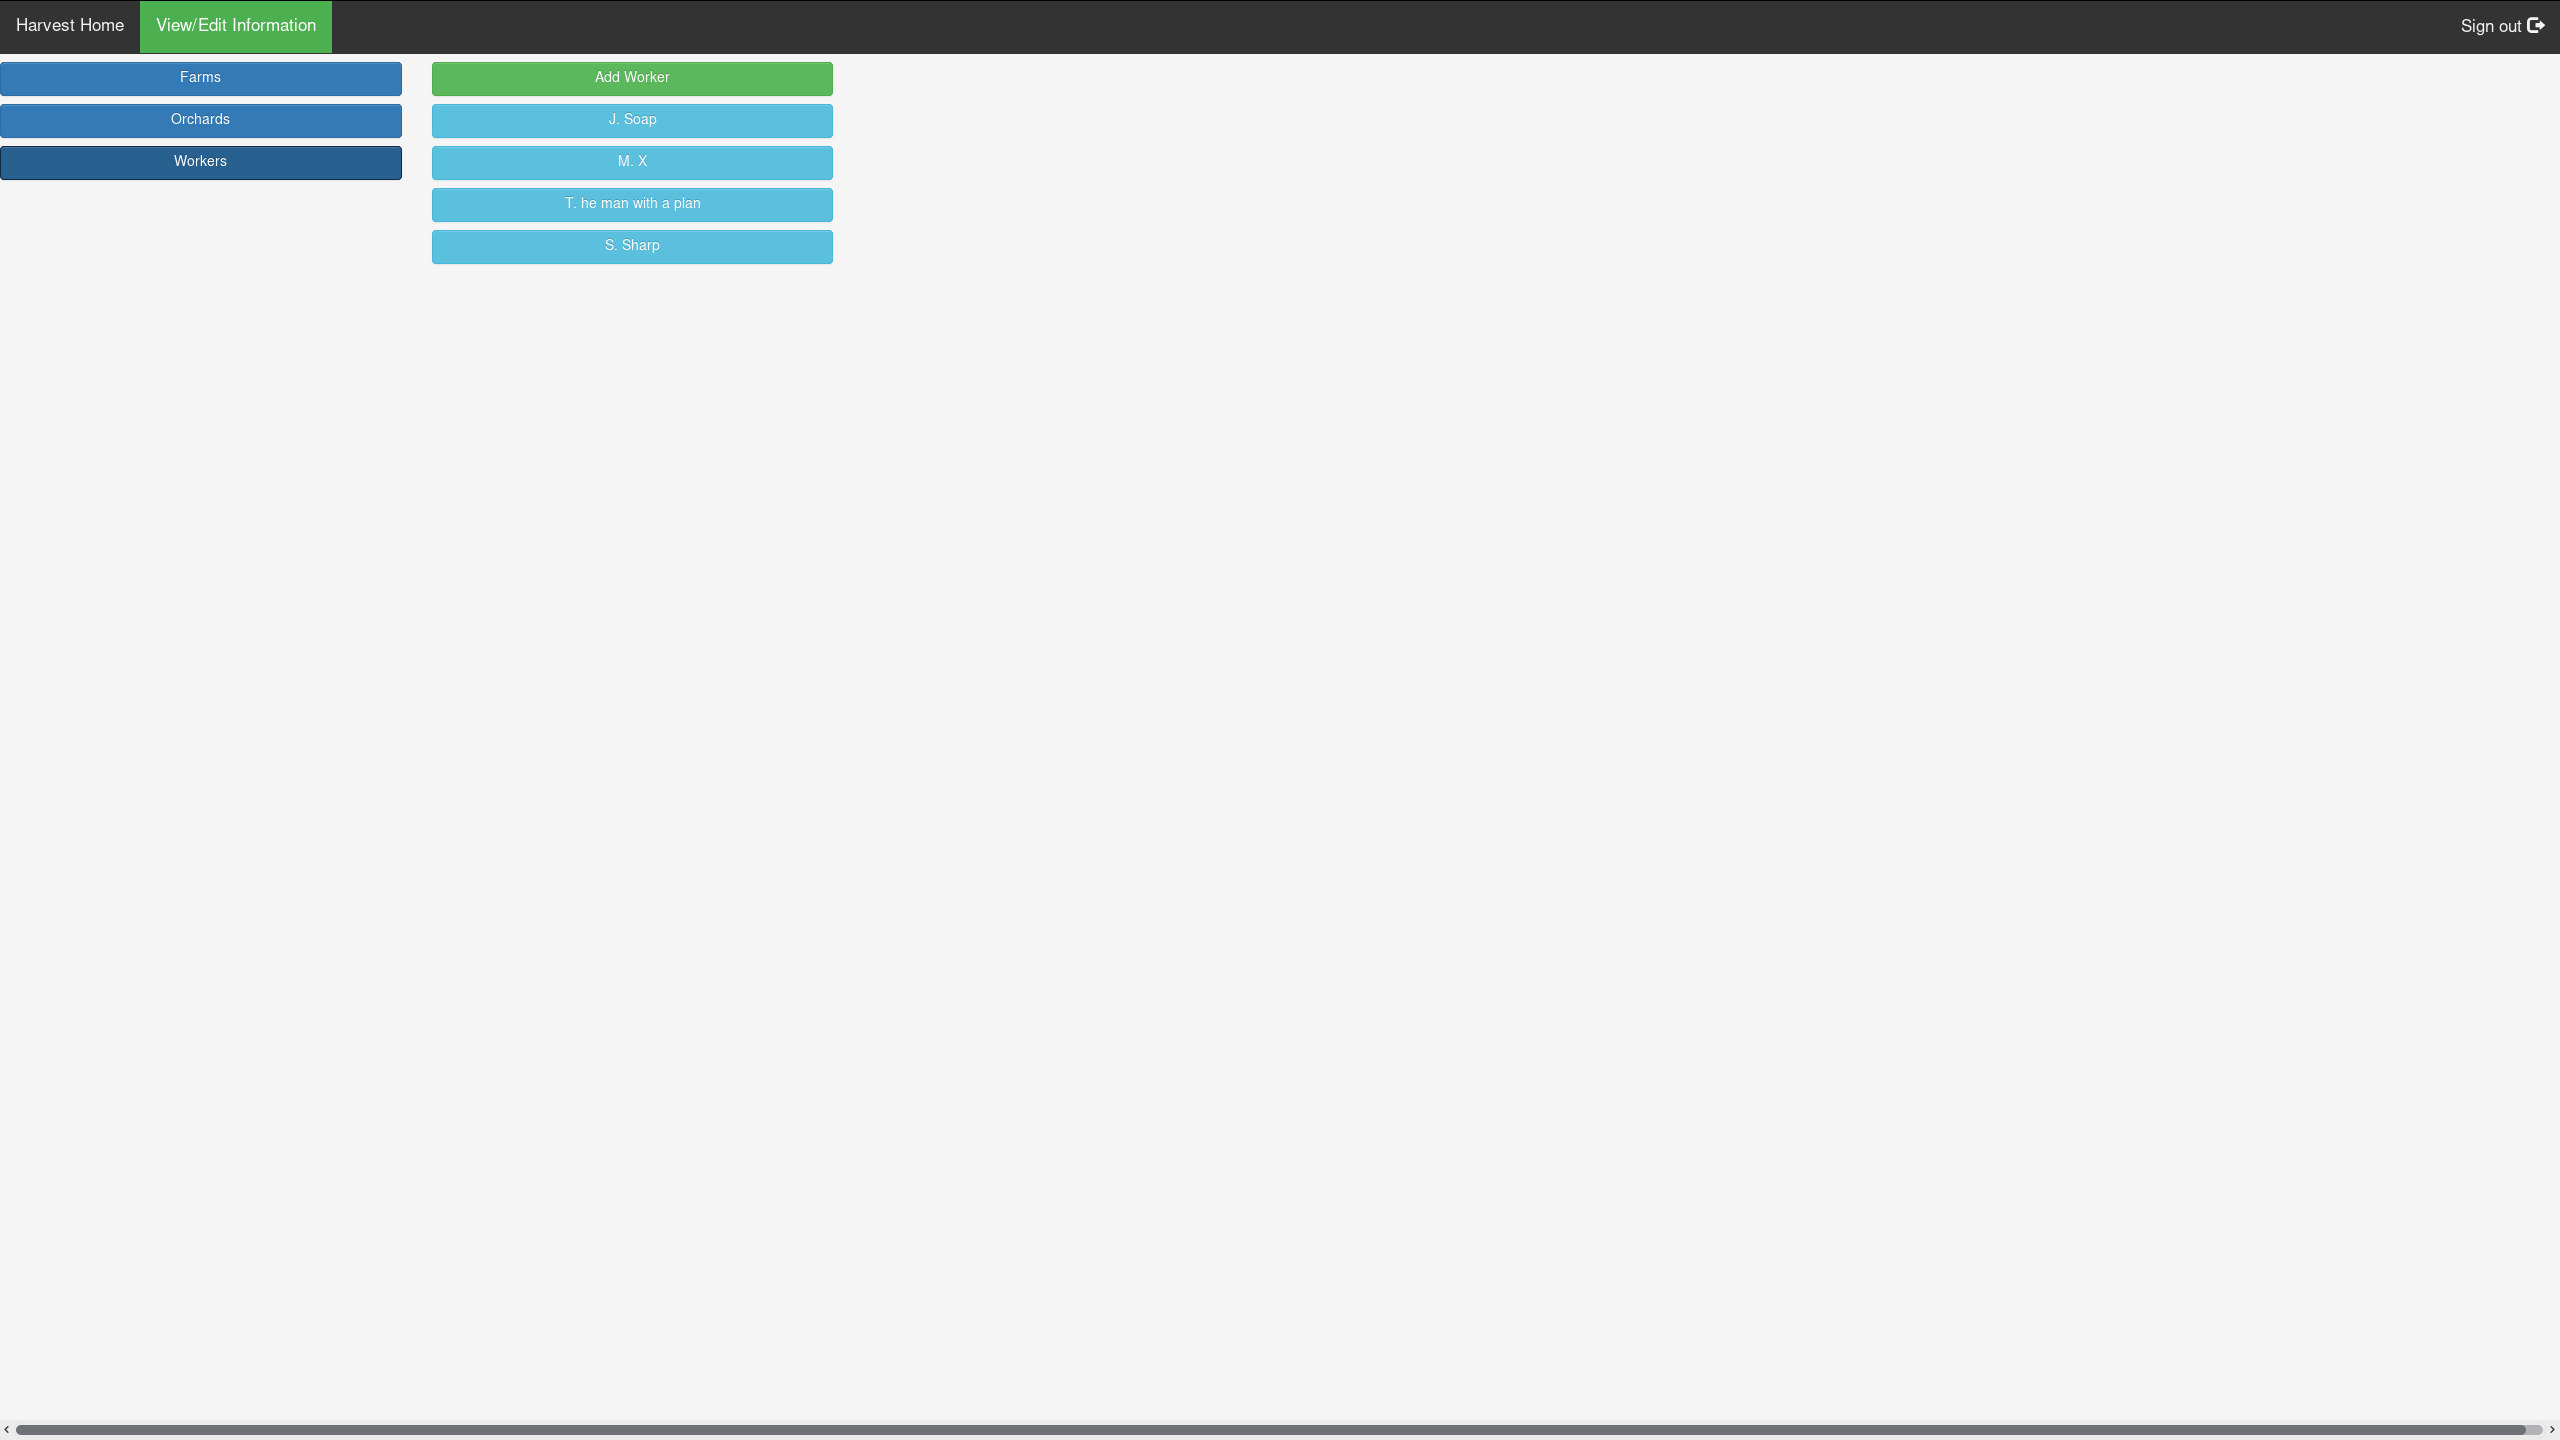
\includegraphics[width=12cm, keepaspectratio]{Images/webInformation-Workers.png}
 \caption{Workers}
 \label{InformationPageWorkers}
\end{figure}

\begin{figure}
 \centering
 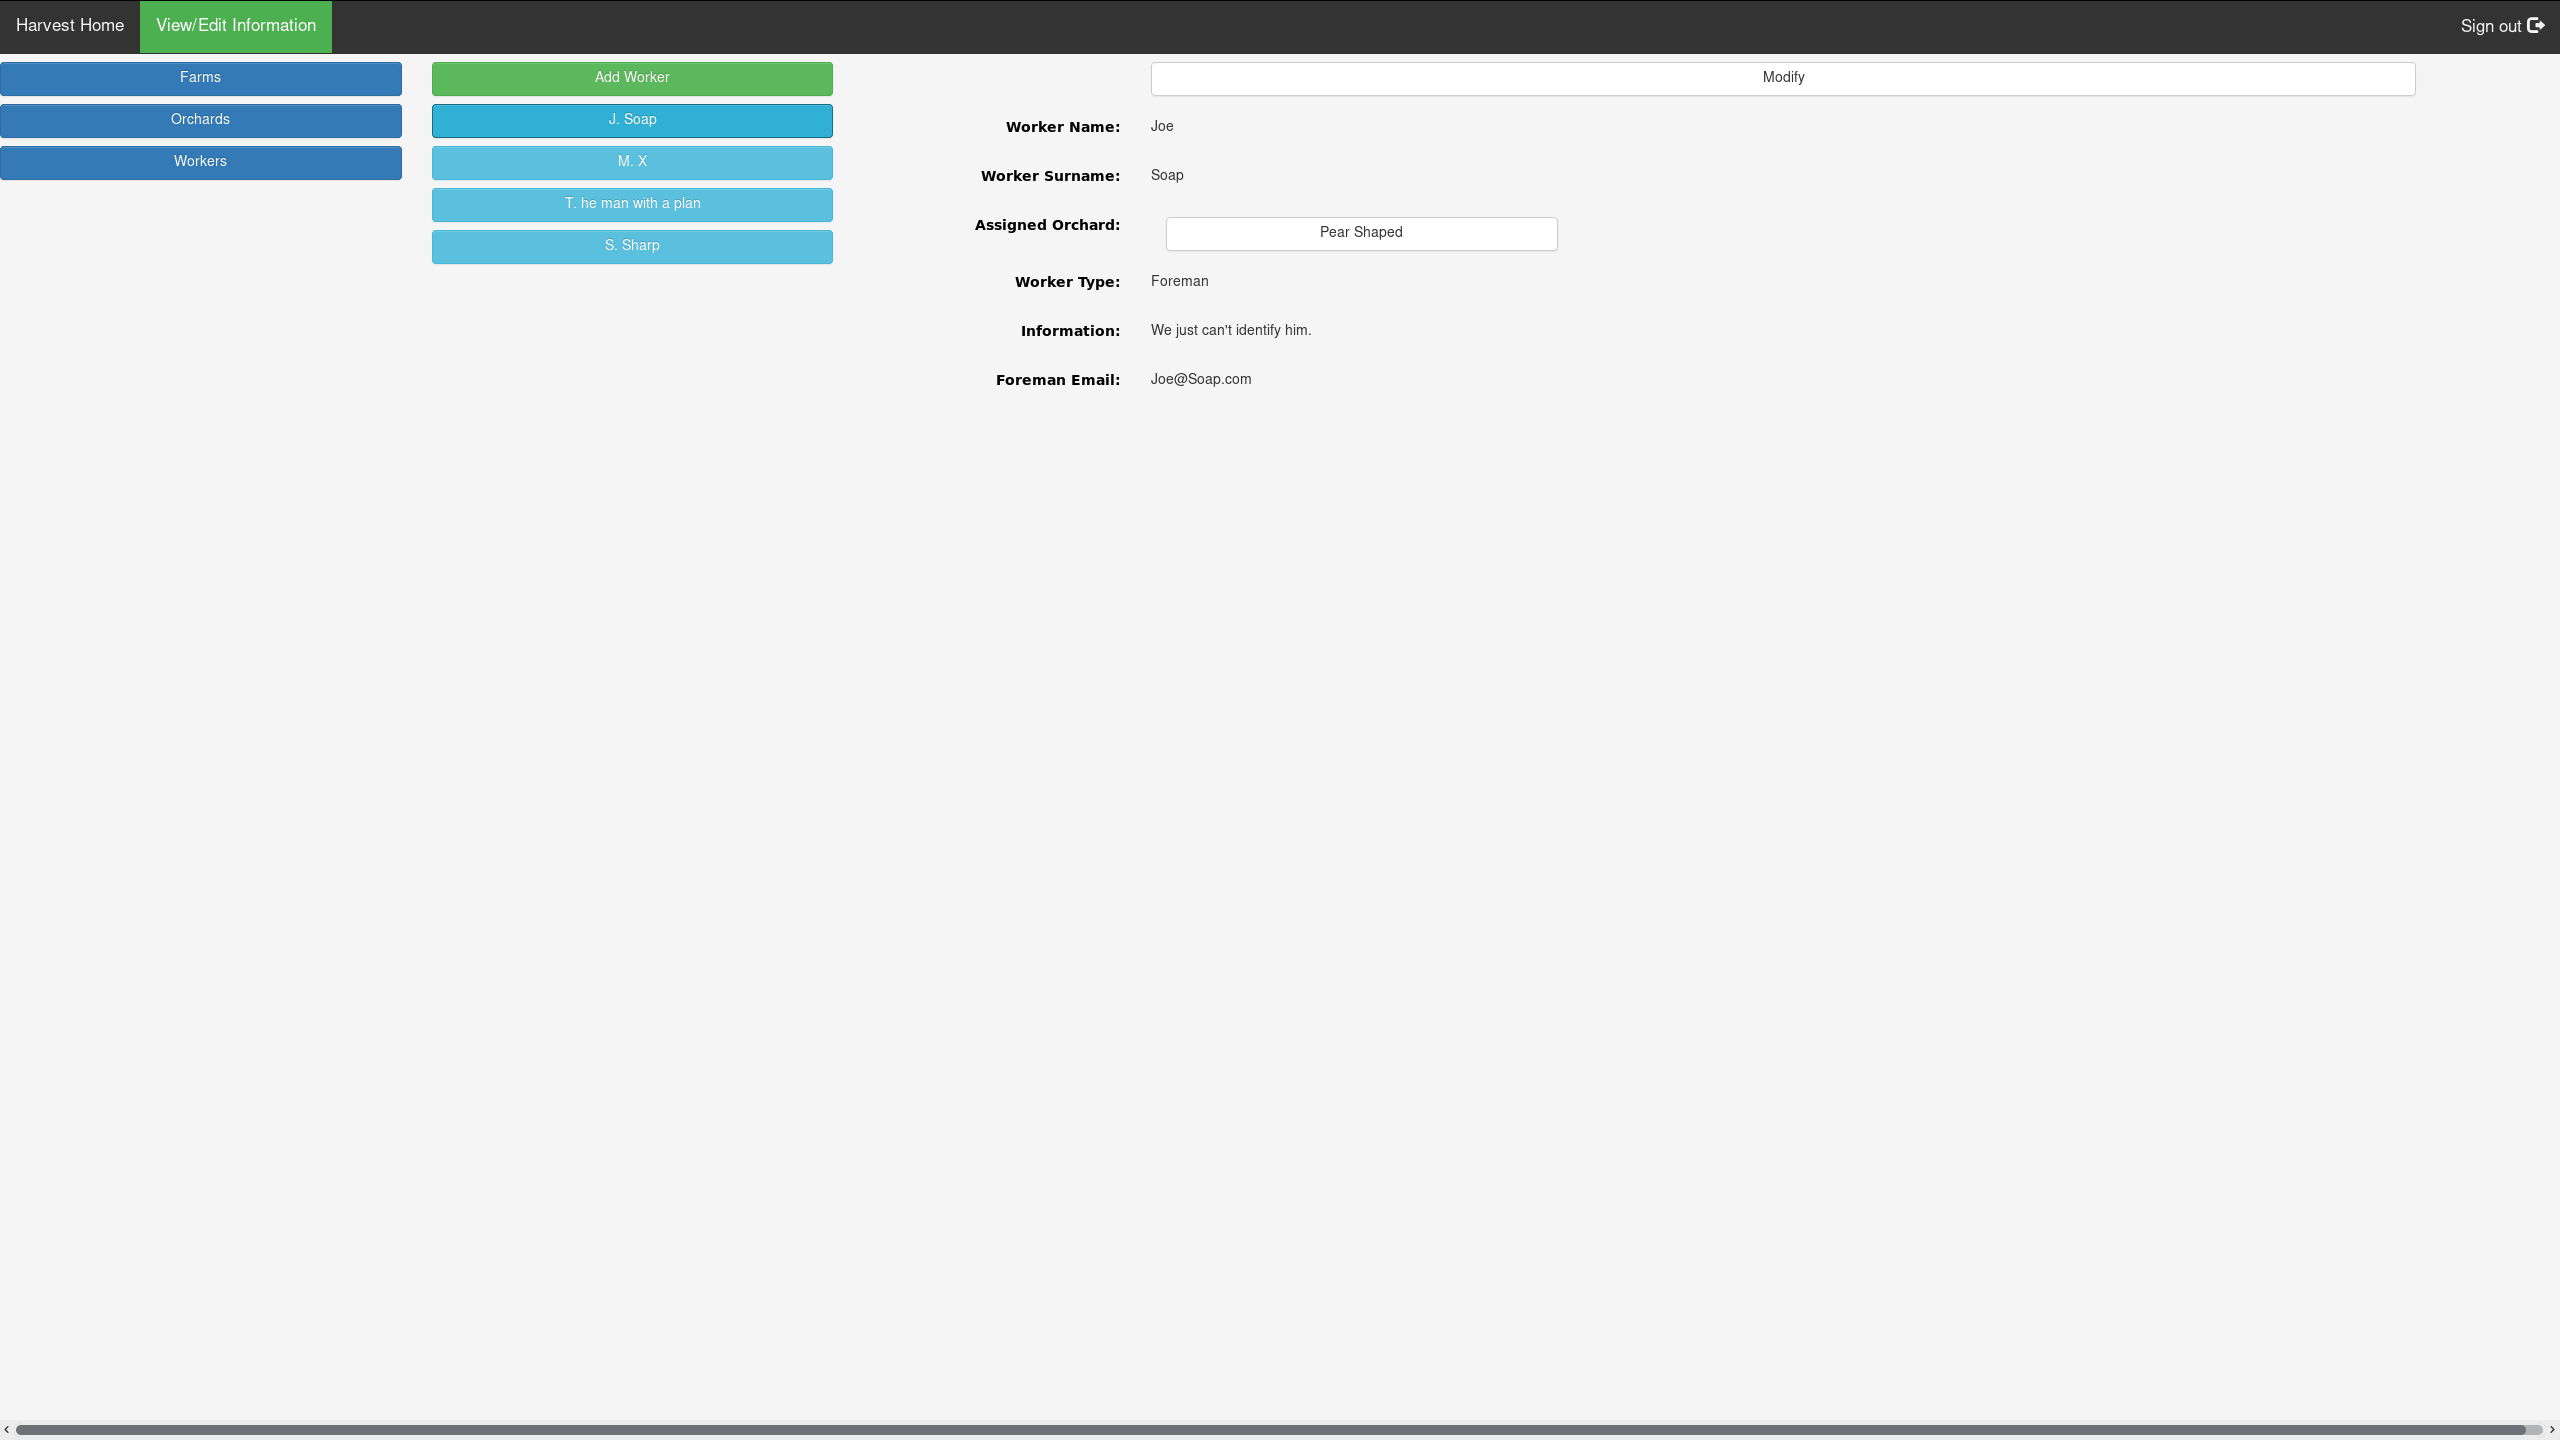
\includegraphics[width=12cm, keepaspectratio]{Images/webInformation-LookWorker.png}
 \caption{Looking at a Worker}
 \label{InformationPageJoe}
\end{figure}

\begin{figure}
 \centering
 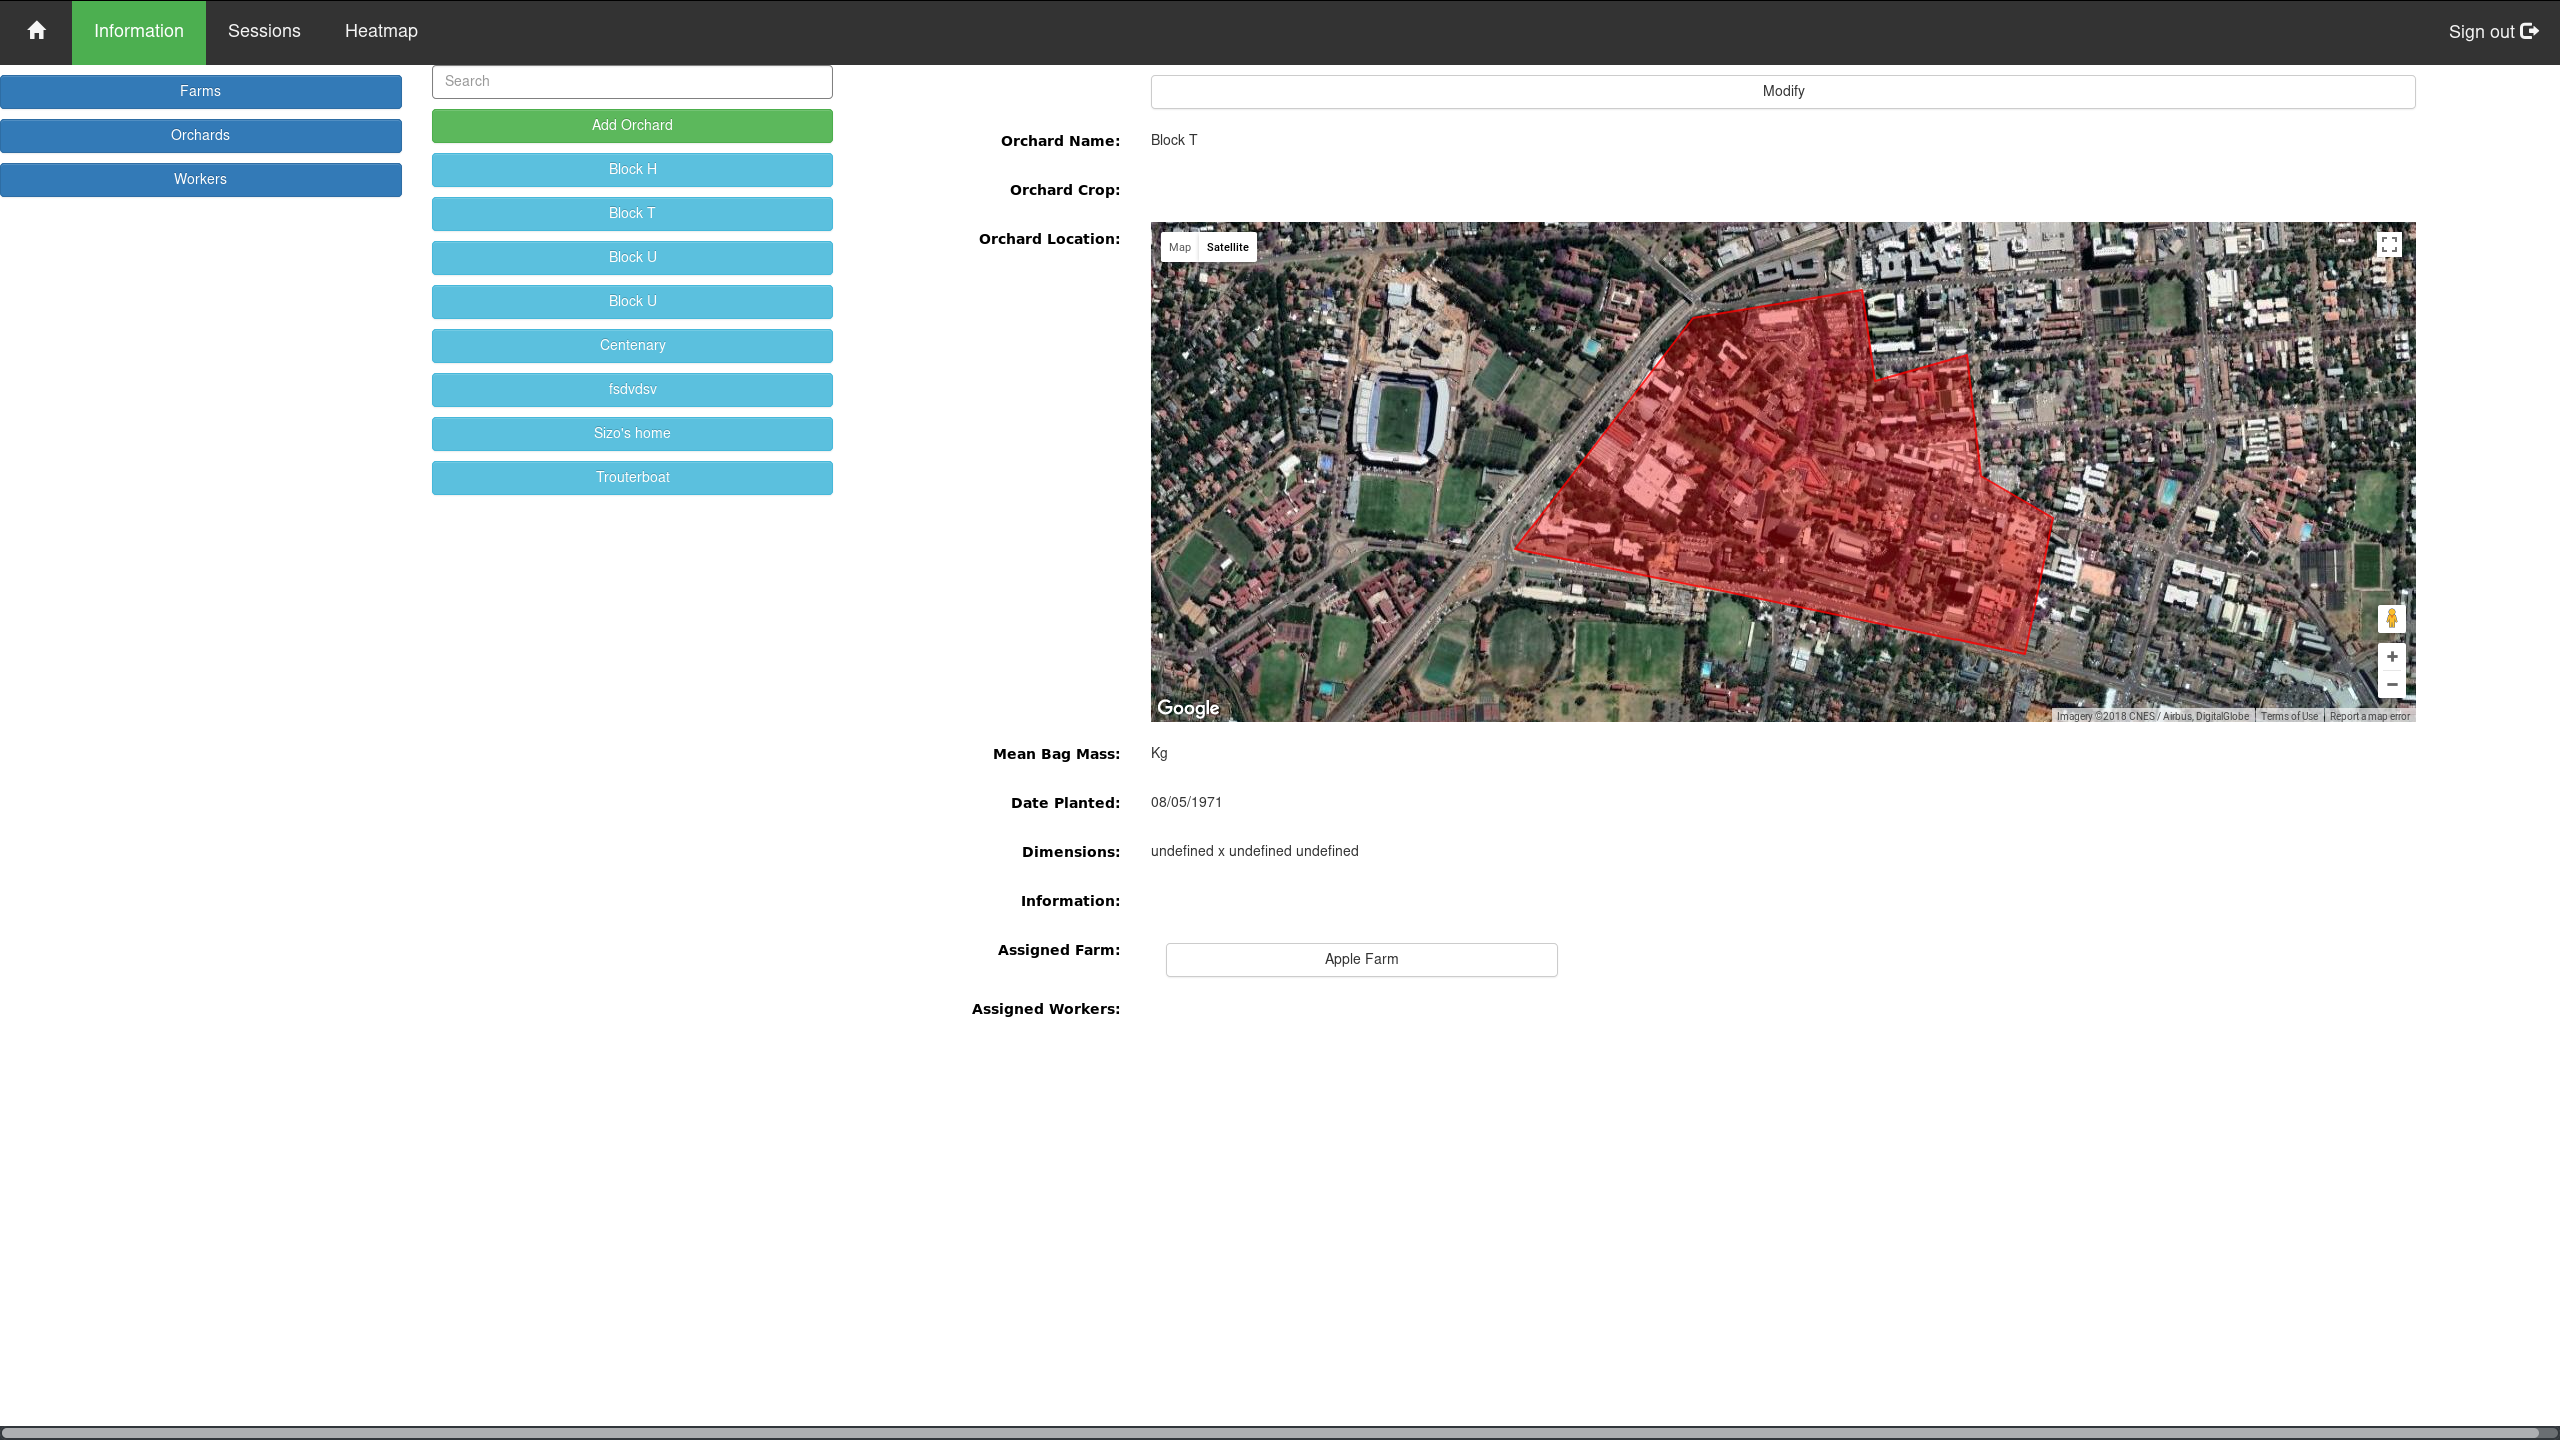
\includegraphics[width=12cm, keepaspectratio]{Images/webViewOrchard.png}
 \caption{Looking at an Orchard}
 \label{InformationPagePear}
\end{figure}

\paragraph{Adding Information}Note that at the top of the second list in \ref{InformationPageWorkers}, \ref{InformationPageJoe}, \ref{InformationPagePear}, or \ref{InformationPageJoePear} there is a green \texttt{Add Farm}, \texttt{Add Orchard}, or \texttt{Add Worker} button, clicking this button will display the interface to enter the necessary information. An example of this can be seen in \ref{InformationAddOrchard}, where a new orchard can be created. Once all of the necessary information has been entered, then the \texttt{Save} button can be clicked to create the new orchard, note that none of the fields are required.

\begin{figure}
 \centering
 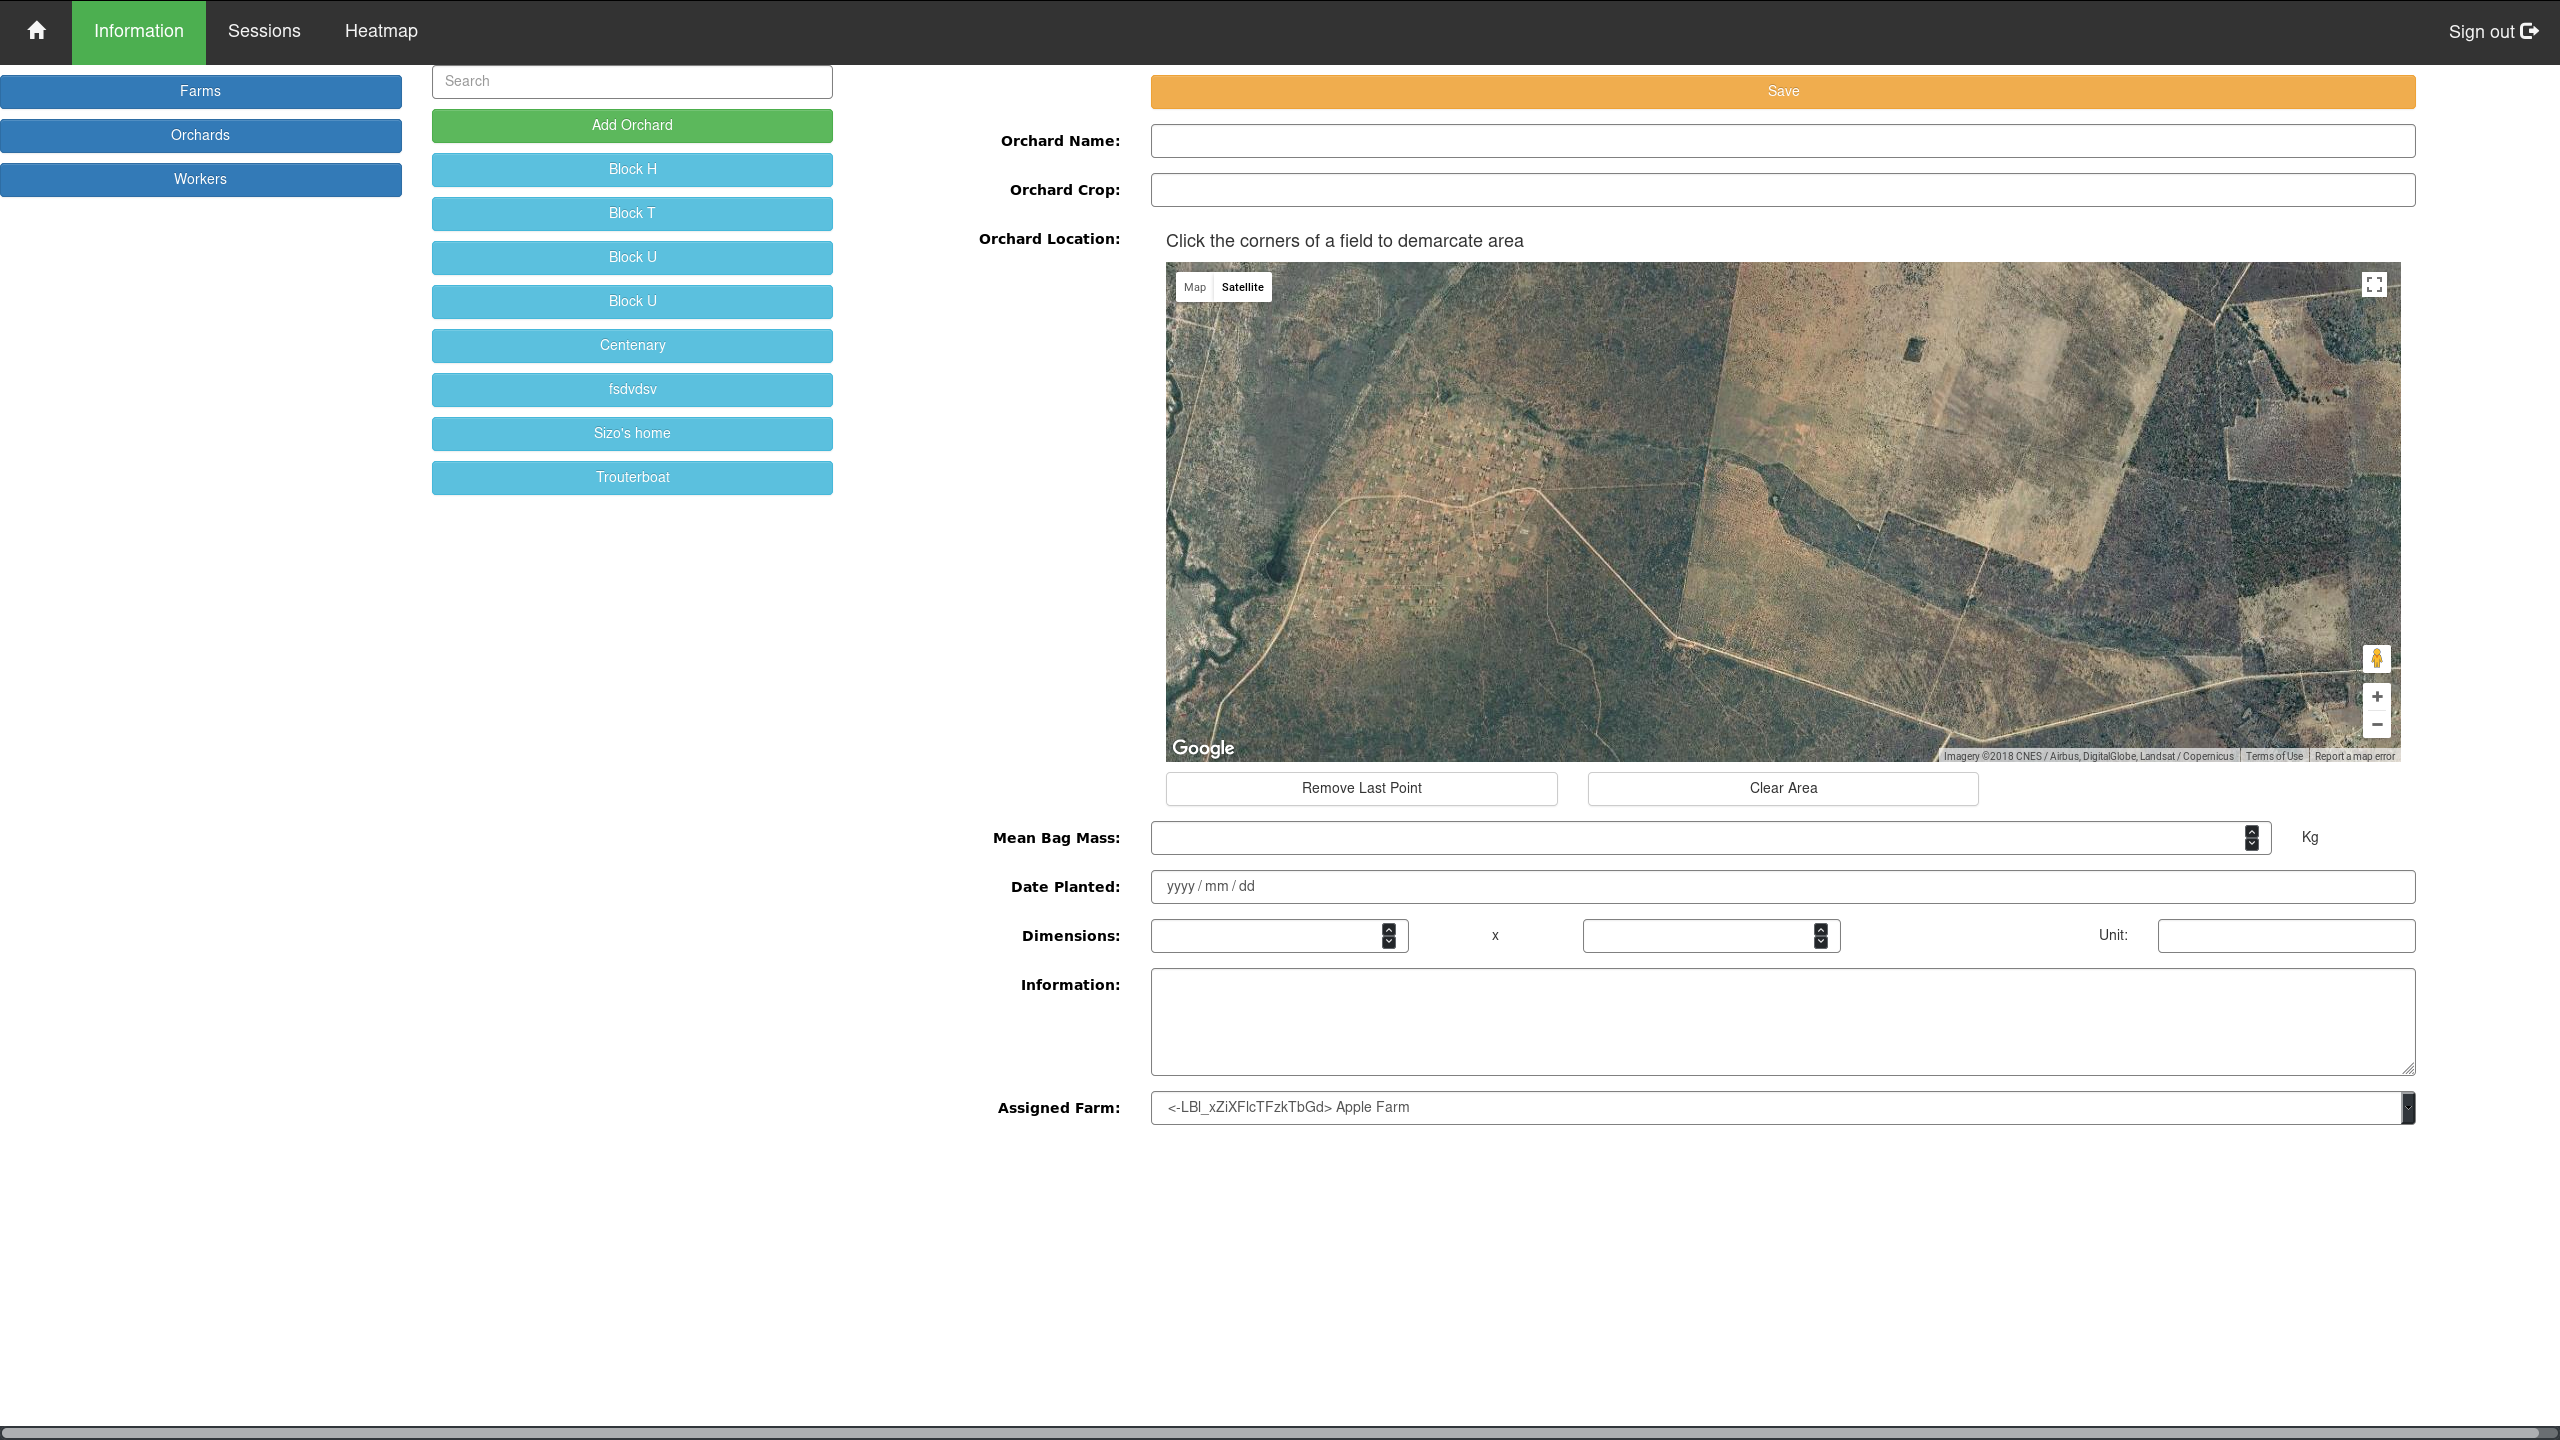
\includegraphics[width=12cm, keepaspectratio]{Images/webInformation-AddOrchard.png}
 \caption{Adding an Orchard}
 \label{InformationAddOrchard}
\end{figure}

\paragraph{Modifying Information}When looking at any information, a \texttt{Modify} button can be seen at the top (see \ref{InformationPageJoe}, \ref{InformationPagePear}, or \ref{InformationPageJoePear}). In \ref{InformationModJoe} the view when \textit{Joe Soap} is being modified can be seen. The fields are already populated by the information that was already stored in them. Once the user is content with the changes, they can click on the orange \texttt{Save} button to apply the changes. A reminder that no fields are required, so that fulled in fields can be erased. The user can also click on the red \texttt{Delete} button to delete the entry in its entirety---note a confirmation dialog will appear. The user may also cancel, which will return them to before they clicked on \texttt{Modify}, as seen in \ref{InformationPageJoe}, \ref{InformationPagePear}, or \ref{InformationPageJoePear}.

\begin{figure}
 \centering
 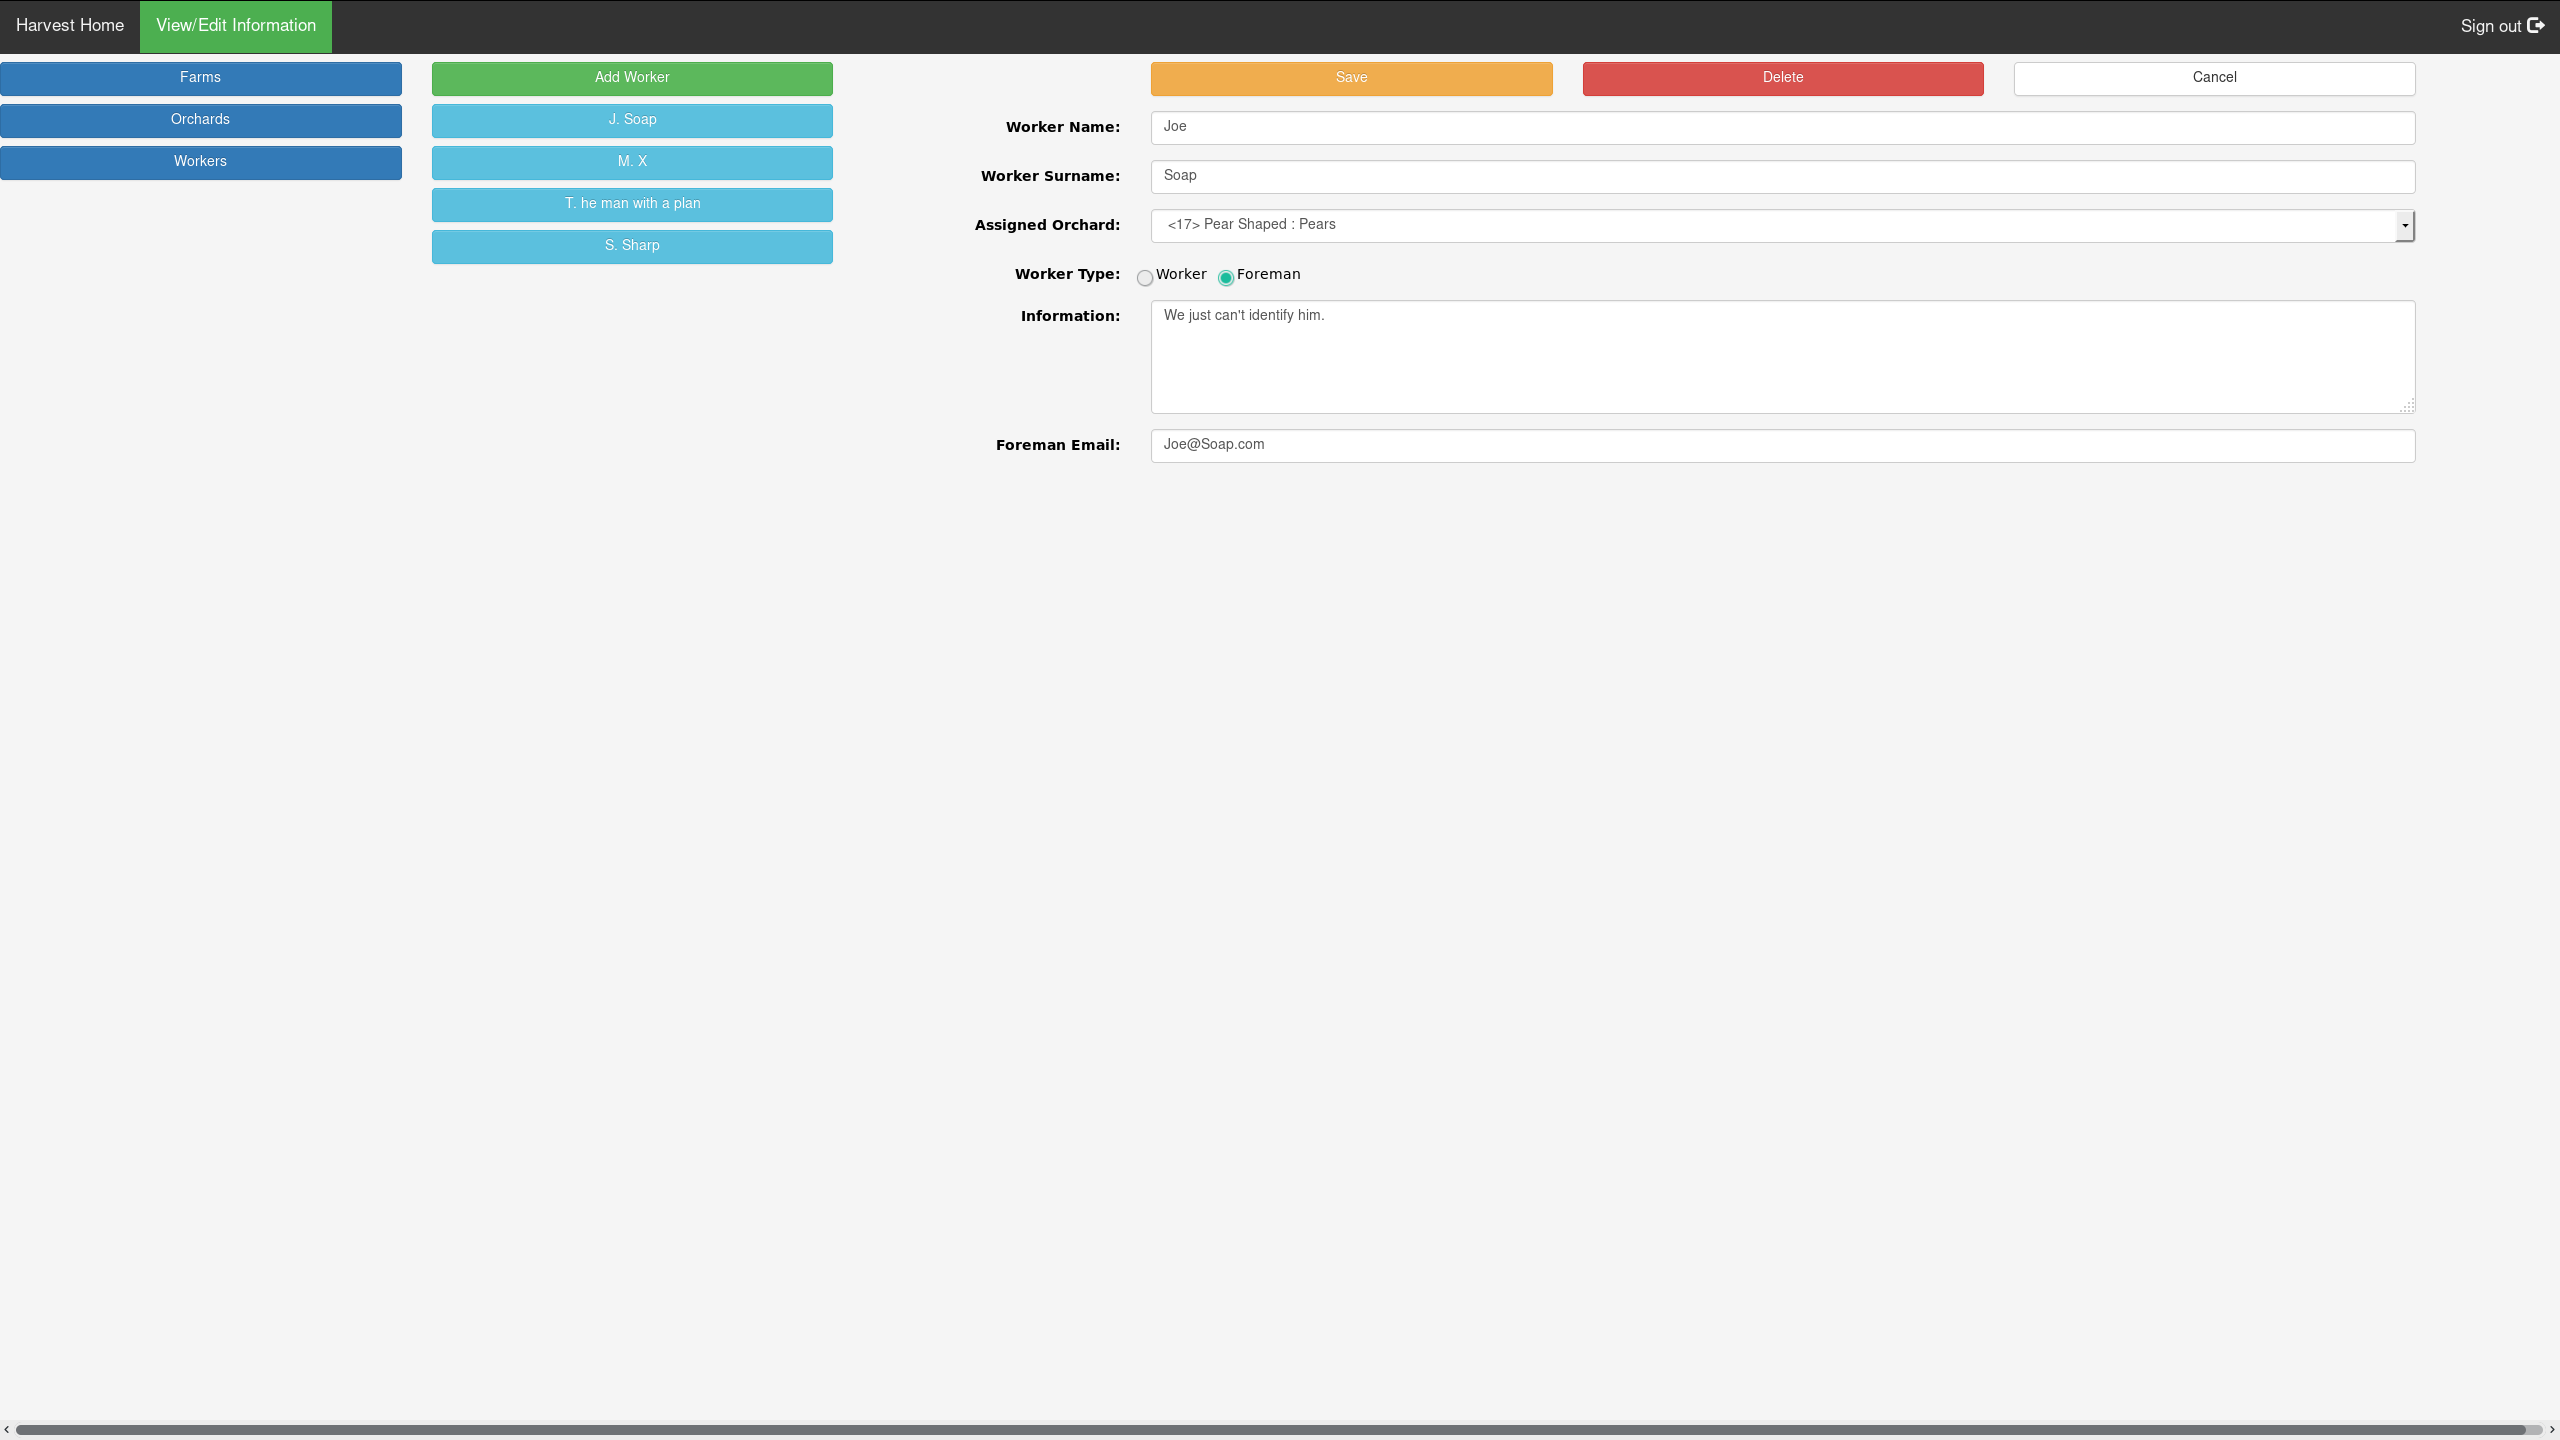
\includegraphics[width=12cm, keepaspectratio]{Images/webInformation-Mod-Worker.png}
 \caption{Modifying a Worker}
 \label{InformationModJoe}
\end{figure}

\paragraph{Stored Information}
Below, the fields stored are described.
\subparagraph{Farm}
\begin{itemize}
 \item \textit{Farm Name}: the name of the farm.
 \item \textit{Information}: any further textual information about the farm.
 \item \textit{Assigned Orchards}: a clickable list of the orchards assigned to the farm.
\end{itemize}

\subparagraph{Orchard}
\begin{itemize}
 \item \textit{Orchard Name}: the name of the orchard.
\item \textit{Orchard Crop}: the type of crop grown in the orchard.
\item \textit{Mean Bag Mass}: the average mass of a bag that is harvested from the orchard.
\item \textit{Date Planted}: the date that the orchard was planted.
\item \textit{Spacing}: the spacing of the crops.
\item \textit{Information}: any further textual information about the orchard.
\item \textit{Assigned Farm}: a clickable button indicating the farm that the orchard is assigned to.
\item \textit{Assigned Workers}: a clickable list of the workers assigned to the orchard.
\end{itemize}

\subparagraph{Worker}
\begin{itemize}
\item \textit{Worker Name}: the first name of the worker.
\item \textit{Worker Surname}: the surname of the worker.
\item \textit{Assigned Orchard}: a clickable button indicating the orchard that the worker is assigned to.
\item \textit{Worker Type}: indicates if the worker is a foreman or a regular worker.
\item \textit{Information}: any further textual information about the worker.
\item \textit{Foreman Email}: in the case of a foreman, their email address for linking to their app.
\end{itemize}
\subsubsection{Sessions}
\label{webSessions}
From here, a list of all sessions can be seen and selected. Once selected, information about the session will be displayed. Above the map the foreman that administered the session; and the time started, and ended; are displayed. The map shows the path taken by the foreman, as well as where they were when they indicated a bag drop. Please see \ref{webSession}. Below the map a pie chart is displayed, showing what portion of the total bags dropped was done by each worker.

\begin{figure}
 \centering
 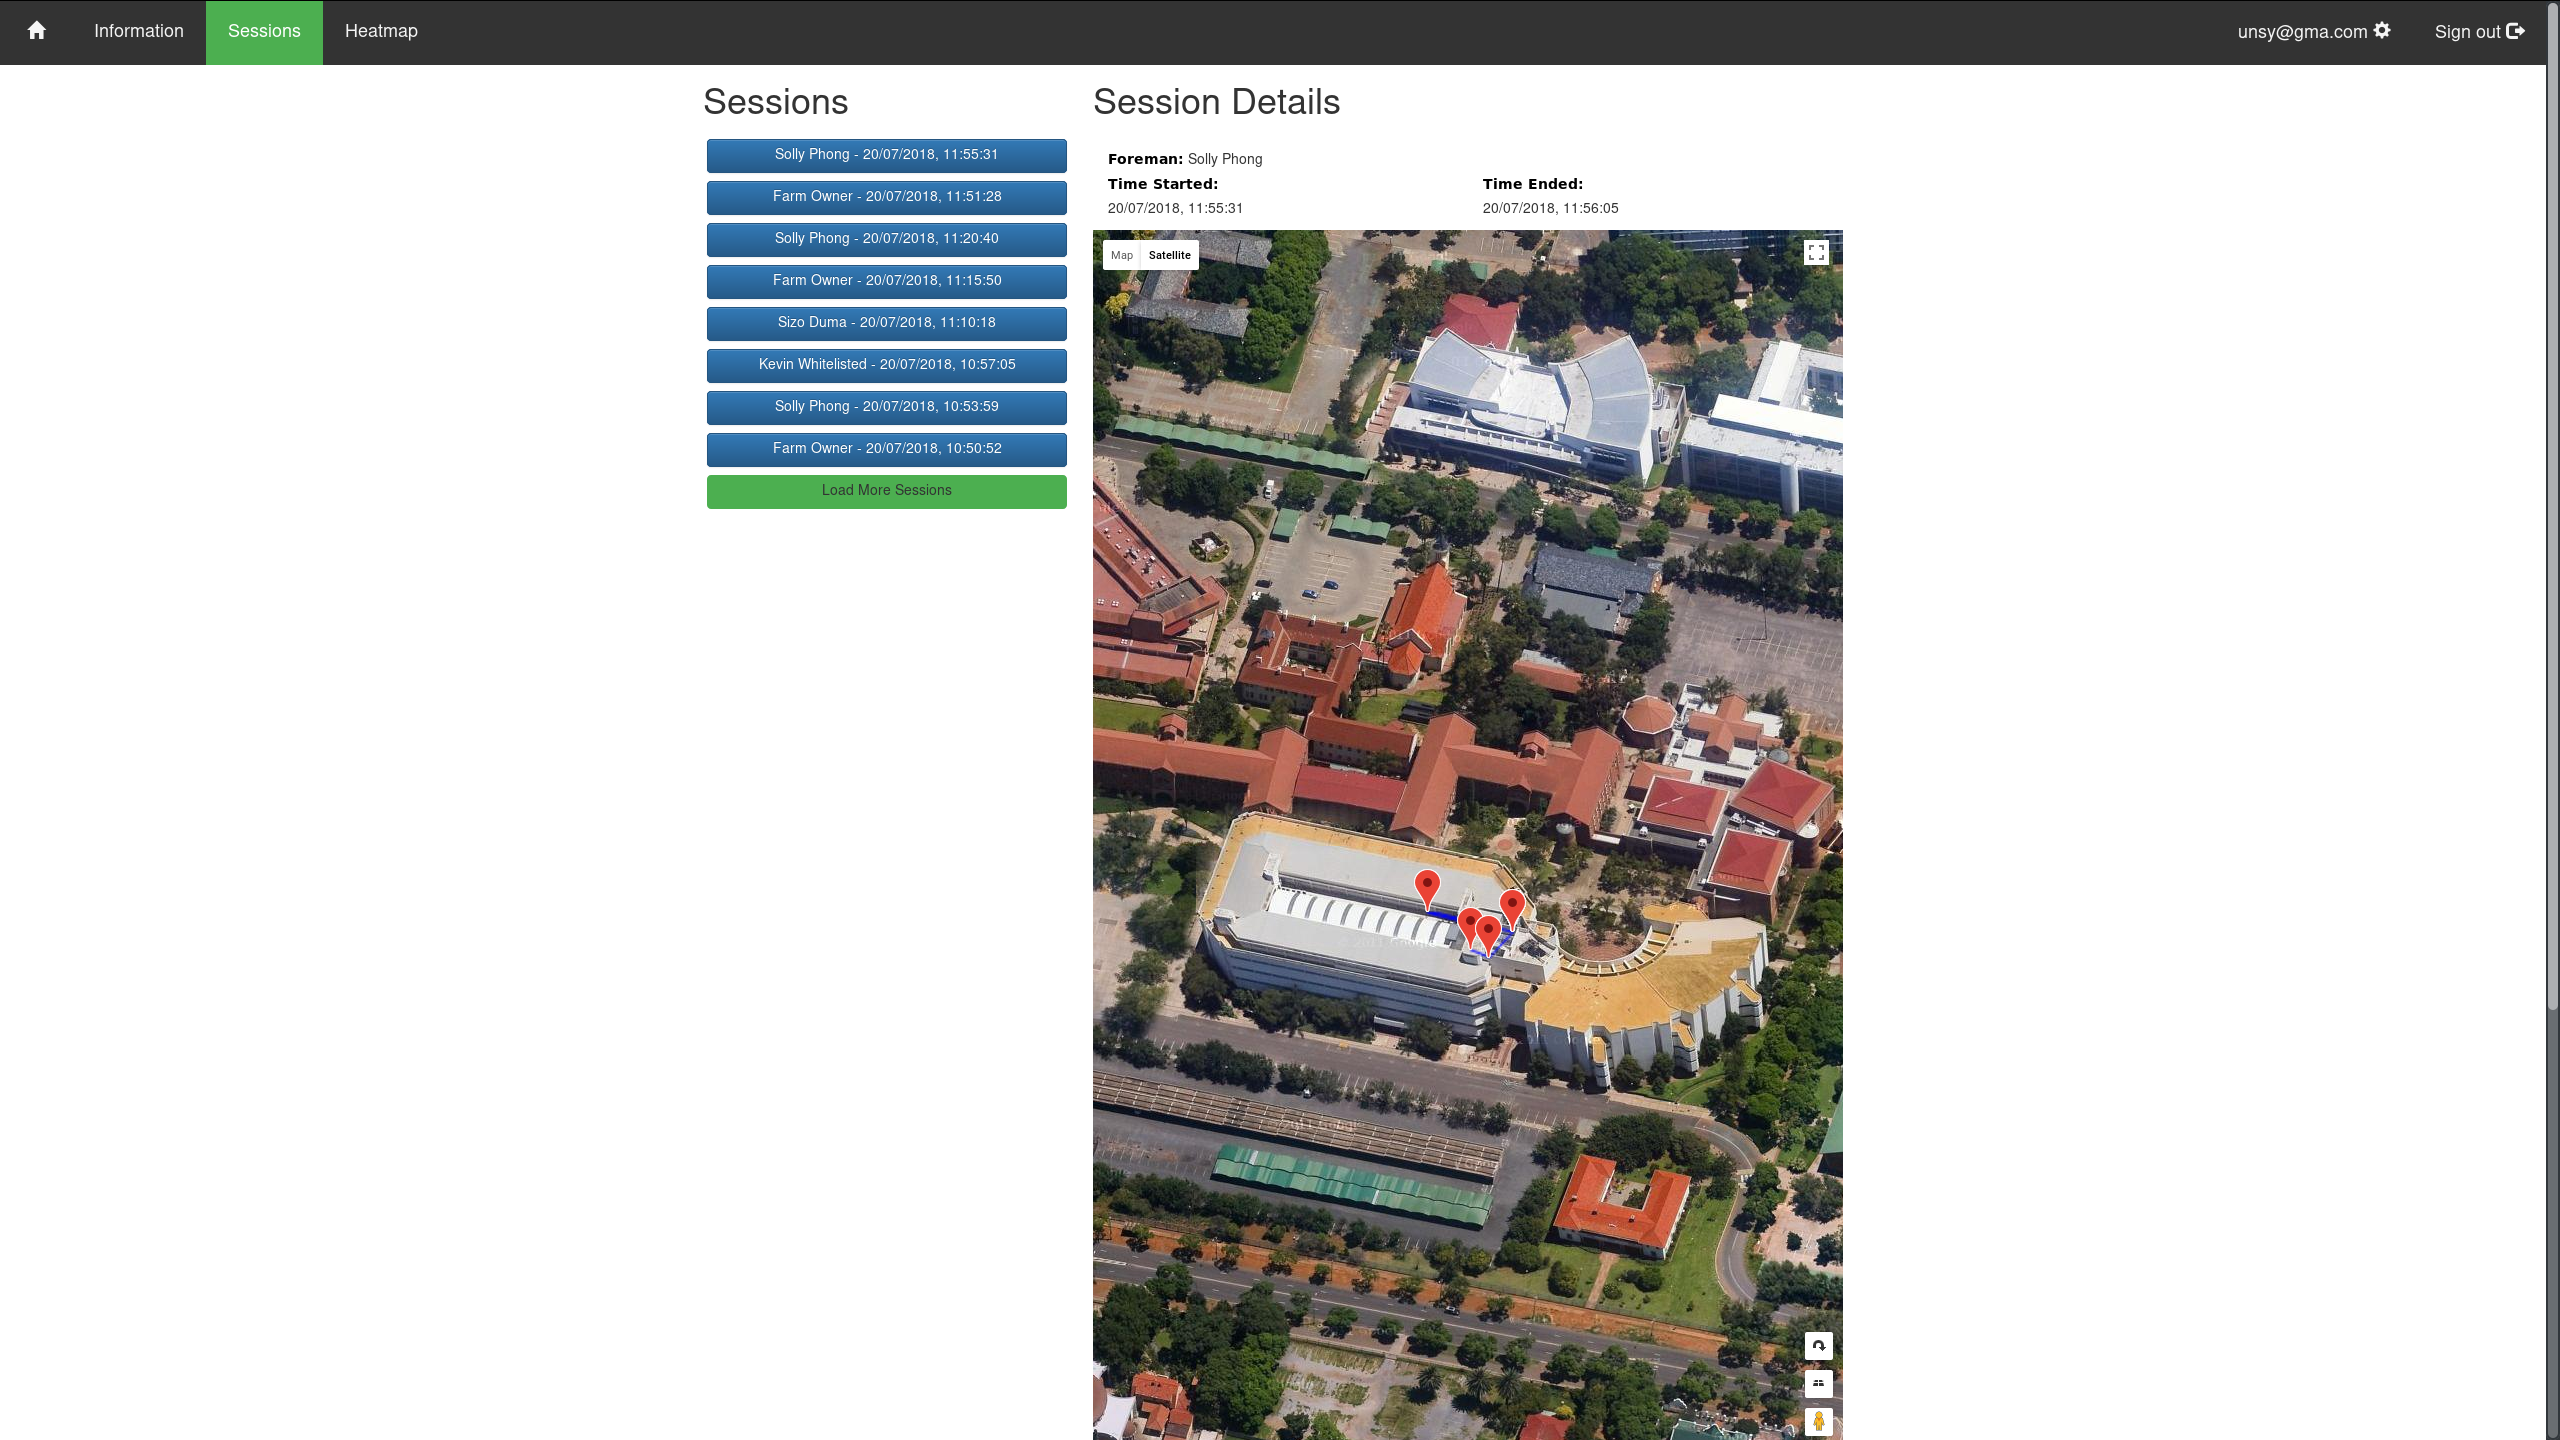
\includegraphics[width=12cm, keepaspectratio]{Images/webSession.png}
 \caption{Session}
 \label{webSession}
\end{figure}

\subsubsection{Heatmap}
\label{webHeatmap}

The heatmap (\ref{webHeatmap}) shows where the majority of bag drops took place, by having more active areas be redder.

\begin{figure}
 \centering
 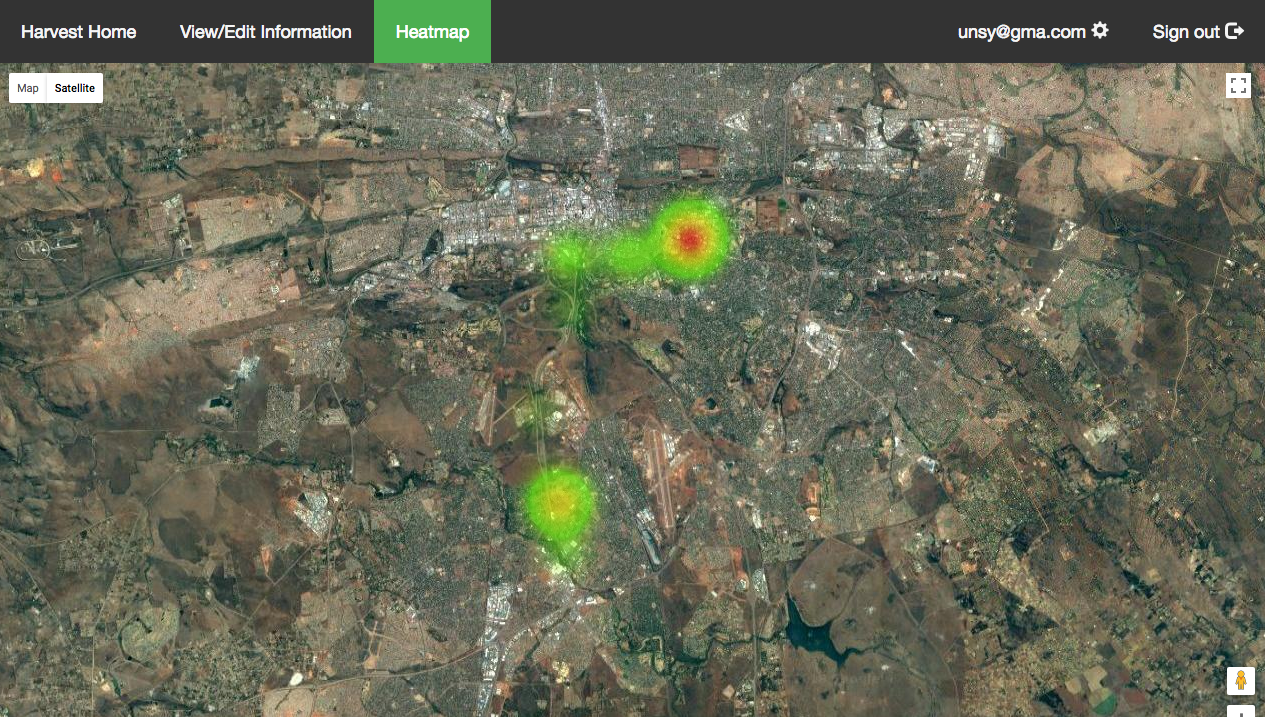
\includegraphics[width=12cm, keepaspectratio]{Images/webHeatMap.png}
 \caption{Heat Map}
 \label{HeatMap}
\end{figure}
\subsubsection{Analytics}
\label{webAnalytics}
\subsubsection{Settings}
\label{webSettings}


\newpage
\section{Troubleshooting}

\subsection{Mobile and Website}

\subsubsection{Forgotten Password}
\begin{enumerate}
\item On the sign in screen, tap "Forgot account details?" button.
\item When asked for your email, enter the the email address of the account with the forgotten password.
\item An email will be sent to that address.
\item Follow the instructions in the email. You will click on a link in the email.
\item From the web page that the link sent you to, Enter the new password for your account.
\item Log in to Harvest using your new details.
\end{enumerate}

\subsection{Mobile Only}
\subsubsection{Location Services}
\begin{enumerate}
\item Check that your phone supports location services
\item In the "Settings" application make sure that the Harvest app is allowed location services 
\end{enumerate}

\subsection{Website Only}

\end{document}
